\documentclass[preview]{standalone}
%\usepackage{prelude}

%%%%%%%%%%%%%%%%%%%%%%%%%%%%%%%%%%%% PACKAGES %%%%%%%%%%%%%%%%%%%%%%%%%%%%%%%%%%%%%%%%%%

\usepackage{inputenc,fontenc}
\usepackage[a4paper,margin=3cm]{geometry}
\usepackage[english]{babel}
%\usepackage[german]{babel}
%\usepackage[fixlanguage]{babelbib}


\usepackage{bbold}
\usepackage{amsthm}
\usepackage{amsmath}
\usepackage{amssymb} % doteqdot
\usepackage[dvipsnames]{xcolor}
\usepackage{standalone}
\usepackage{tikz}[mode=buildnew]
\usepackage{cite}
\usepackage{xspace}
\usepackage{relsize}
\usepackage{mathtools} % mathclap
%\usepackage{MnSymbol}
\usepackage{hyperref}
\usepackage{url}
\usepackage{listings} % for code
\usepackage[T1]{fontenc} %<
\hypersetup{
	colorlinks,
	citecolor=black,
	filecolor=black,
	linkcolor=black,
	urlcolor=black
}
\usepackage{pgfplots}
\pgfplotsset{compat=1.18}
%\usepackage{courier} %% Sets font for listing as Courier. But also for url and texttt!
\usepackage{listings, xcolor}
\usepackage{graphicx}
\usepackage{subcaption}

\usetikzlibrary{calc}
%\usepackage{xparse} % \newDocumentCommand for multiple optional arguments
%\usepackage{titlecaps}



%%%%%%%%%%%%%%%%%%%%%%%%%%%%%%%%%%%% THEOREMSTYLES %%%%%%%%%%%%%%%%%%%%%%%%%%%%%%%%%%

\theoremstyle{definition}
\newtheorem{definition}{Definition}[section]
\newtheorem{exmp}{Beispiel}[section]
%\AfterEndEnvironment{definition}{\noindent\ignorespaces}

\theoremstyle{theorem}
\newtheorem{theorem}{Satz}[section]
\newtheorem{proposition}{Proposition}[section]
%\AfterEndEnvironment{theorem}{\noindent\ignorespaces}

\theoremstyle{korollary}
\newtheorem{korollary}{Korollar}[section]
%\AfterEndEnvironment{korollary}{\noindent\ignorespaces}


\tikzset{
	mstate/.style={draw, circle, minimum size=.94cm}, 
	gstate/.style={draw, rectangle, minimum size=.8cm},
	varstate/.style={draw,rectangle, rounded corners, minimum size=1}, 
	trans/.style={draw, ->, thick},
	bendtrans/.style={draw, ->, thick, bend left=10},
	bendtransr/.style={draw, ->, thick, bend right=10},
	init/.style={initial, initial distance=6pt, initial text=},
	every loop/.style={min distance=5pt, looseness=8},
	>=latex
}
\usetikzlibrary{automata,positioning}

%auto shift/.style={auto=right,->,
%	to path={ let \p1=(\tikztostart),\p2=(\tikztotarget),
%		\n1={atan2(\y2-\y1,\x2-\x1)},\n2={\n1+180}
%		in ($(\tikztostart.{\n1})!1mm!270:(\tikztotarget.{\n2})$) -- 
%		($(\tikztotarget.{\n2})!1mm!90:(\tikztostart.{\n1})$) \tikztonodes}},

%%%%%%%%%%%%%%%%%%%%%%%%%%%%%%%%%%% MY MACROS %%%%%%%%%%%%%%%%%%%%%%%%%%%%%%%%%%%%%%%%%
%formatting
\newcommand{\comment}[2]{{\color{#1}#2}}
\newcommand{\redcomment}[1]{{\color{red}#1}}
\newcommand{\purpcomment}[1]{{\color{pink}#1}}
\newcommand{\bluecomment}[1]{{\color{blue}#1}}
\newcommand{\mt}[1]{\ensuremath{{#1}}\xspace}
\newcommand{\mynewcommand}[2]{\newcommand{#1}{\mt{#2}}} %% currently not used becaue of ide highlighting
\newcommand{\arr}{\mt{\to}}

%model checking terms
\newcommand{\mimicrel}{\mt{\mathcal{R}}}
\newcommand{\bisimeq}{\mt{\;\!\sim\;\!}}
\newcommand{\simorder}{\mt{\;\!\preceq\;\!}}
\newcommand{\simequiv}{\mt{\;\!\simeq\;\!}} %command already defined
\newcommand{\relts}{\mt{\;\!\bullet_{_{\tiny{TS}}}\;\!}}
\newcommand{\rel}{\mt{\;\!\bullet\;\!}}

%own names
\newcommand{\nm}[1]{#1\xspace}
\newcommand{\mdpN}{\nm{MDP}}
\newcommand{\mdpsN}{\nm{MDPs}}
\newcommand{\viewN}{\nm{view}}
\newcommand{\viewNC}{\nm{View}}
\newcommand{\viewsN}{\nm{views}}
\newcommand{\viewsNC}{\nm{Views}}
\newcommand{\grpfctsubN}{\nm{detached grouping function}}
\newcommand{\grpfctsubNC}{\nm{detached grouping function}}
\newcommand{\grpfctsubNCC}{\nm{Detached Grouping Function}}
\newcommand{\grpfctN}{\nm{grouping function}}
\newcommand{\grpfctNC}{\nm{Grouping function}}
\newcommand{\grpfctNCC}{\nm{Grouping Function}}
\newcommand{\grpfctsN}{\nm{grouping functions}}
\newcommand{\grpfctsNC}{\nm{Grouping functions}}
\newcommand{\grpfctsNCC}{\nm{Grouping Functions}}
\newcommand{\stmimicN}{\nm{state-mimic}}
\newcommand{\stmimicsN}{\nm{state-mimics}}
\newcommand{\stmimickingN}{\nm{state-mimicking}}
\newcommand{\stmimickedN}{\nm{state-mimicked}}
%\newcommand{\chosenphtypeNCC}{\nm{Transition System}}
%\newcommand{\chgphNC}{\nm{Transition system}}
%\newcommand{\chgphN}{\nm{transition system}}
%\newcommand{\chgphsNCC}{\nm{Transition Systems}}
%\newcommand{\chgphsNC}{\nm{Transition systems}}
%\newcommand{\chgphsN}{\nm{transition systems}}
\newcommand{\chgphNCC}{\nm{MDP}}
\newcommand{\chgphNC}{\nm{MDP}}
\newcommand{\chgphN}{\nm{MDP}}
\newcommand{\achgphN}{\nm{an MDP}}
\newcommand{\chgphsNCC}{\nm{MDPs}}
\newcommand{\chgphsNC}{\nm{MDPs}}
\newcommand{\chgphsN}{\nm{MDPs}}
\newcommand{\parllcompN}{\nm{parallel composition}}
\newcommand{\parllcompNC}{\nm{Parallel composition}}
\newcommand{\parllcompNCC}{\nm{Parallel Composition}}
\newcommand{\parllcompsN}{\nm{parallel compositions}}
\newcommand{\parllcompsNC}{\nm{Parallel compositions}}
\newcommand{\parllcompsNCC}{\nm{Parallel Compositions}}
\newcommand{\sccN}{\nm{SCC}}
\newcommand{\sccsN}{\nm{SCCs}}
\newcommand{\bsccN}{\nm{BSCC}}
\newcommand{\bsccsN}{\nm{BSCCs}}
\newcommand{\jgrapht}{\nm{jGraphtT}}

\newcommand{\outactident}{\nm{OutActionsIdent}}

%names
\newcommand{\iffN}{\nm{if and only if}}
\newcommand{\tsN}{\nm{TS}}

%% outactions identical
\newcommand{\outactidentstrong}{\nm{strong}}
\newcommand{\outactidentweak}{\nm{weak}}

% CORE DEFINITIONS
\newcommand{\grpfct}[1][\viewppty]{\mt{F_{#1}}}
\newcommand{\grpfctsub}[1][\viewppty]{\mt{\tilde{F}_{#1}}}
%\newcommand{\grpfctimg}[1]{\mt{{\grpfct}[{#1}]}}
%\newcommand{\fctimg}[2]{\mt{{#1}[{#2}]}}
\newcommand{\eqrelview}{\mt{R}}
\newcommand{\eqclassv}[1][\state]{\mt{\eqclass{#1}{\eqrelview}}}
\newcommand{\eqclasssetv}[1][\states]{\mt{{#1}/\eqrelview}} %OLD: \bigcup_{\state \in \states} \eqclassv
\newcommand{\viewid}{\mt{\mdp}}
\newcommand{\view}[1][\viewppty]{\mt{\viewid_{#1}}}
\newcommand{\imggrp}{\mt{\arbset}}
\newcommand{\imggrpsub}{\mt{X}}
\newcommand{\viewppty}{\mt{\theta}}
\newcommand{\pll}{\mt{\;\!\pllpure\;\!}}
\newcommand{\pllrev}{\mt{\pllpure^{-1}}}
\newcommand{\pllpure}{\mt{||}}
\newcommand{\compselectset}{\mt{Z}}
\newcommand{\compselectpure}{\mt{\pllpure_\compselectset}}
\newcommand{\compselect}{\mt{\;\pllpure_\compselectset\;}}
\newcommand{\remstates}{\mt{\bigcup_{\state \in \states \setminus \states_1}\{\{\state\}\}}}
\newcommand{\nogroupstates}[1][\states_2]{\mt{\bigcup_{\state \in \states \setminus {#1}}\{\{\state\}\}}}
\newcommand{\remelem}{\mt{\bullet}}
\newcommand{\nogroupset}{\mt{\xi}}
\newcommand{\remset}{\mt{\{\remelem\}}}
\newcommand{\gfctpll}{\mt{\grpfct[\pll]}}
\newcommand{\group}{\mt{\top}}
\newcommand{\imggrpbinview}{\mt{\{\remelem, \notppty\}}}
\newcommand{\viewappset}{\mt{\tilde{\states}}}
\newcommand{\hasppty}{\mt{\top}}
\newcommand{\notppty}{\mt{\bot}}
\newcommand{\disregardelem}{\mt{\Delta}}
\newcommand{\disregardelements}{\mt{{\disregardelem_1, \dots, \disregardelem_n}}}



%\newcommand{\mdp}{def}\mdp
%\newcommand{\mdpdef}



% EXAMPLE VIEWS
\newcommand{\pptyatomicprops}{\mt{\atomicprops}}
\newcommand{\pptyinitstates}{\mt{\initstates}}
\newcommand{\pptyinactsetsize}{\mt{|\inacts(\state)|}}
\newcommand{\pptyhasoutact}{\mt{\exists\outact}}
\newcommand{\pptyminoutact}[2]{\mt{#1\leq#2}}
\newcommand{\pptymaxoutact}[2]{\mt{#2\leq#1}}
\newcommand{\pptyspanoutact}[3]{\mt{#1\leq#2\leq#3}}
\newcommand{\pptyoutactsetsize}{\mt{|\outacts(\state)|}}
\newcommand{\pptyoutactsingle}{\mt{|\outacts(\state)|_1}}
\newcommand{\pptystrongoutactident}{\mt{\outacts(\state)_=}}
\newcommand{\pptyweakoutactident}{\mt{\outacts(\state)_\approx}}
\newcommand{\pptyhasinact}{\mt{\exists\inact}}
\newcommand{\pptymininact}[2]{\mt{#1\leq#2}}
\newcommand{\pptymaxinact}[2]{\mt{#2\leq#1}}
\newcommand{\pptyspaninact}[3]{\mt{#1\leq#2\leq#3}}
\newcommand{\pptyinactsingle}{\mt{|\inacts(\state)|_1}}
\newcommand{\pptystronginactident}{\mt{\inacts(\state)_=}}
\newcommand{\pptyweakinactident}{\mt{\inacts(\state)_\approx}}
\newcommand{\pptyparamvalueseq}{\mt{\var = \varval}}
\newcommand{\pptyparamvaluesneq}{\mt{\var \neq \varval}}
\newcommand{\pptyparamdnf}{\mt{VarDNF}}
\newcommand{\pptyparamcnf}{\mt{VarCNF}}
\newcommand{\pptyparamvalueseqopt}{\mt{\var = \varval}}
\newcommand{\pptyparamvalident}{\mt{Var:\varval}}
\newcommand{\pptydistance}{\mt{\distpath}}
\newcommand{\pptydistancerev}{\mt{\distpathrev}}
\newcommand{\pptydistancebi}{\mt{\distpathbi}}
\newcommand{\pptyhascycle}{\mt{\exists\cycle}}
\newcommand{\pptyexactactcycle}{\mt{\{\cycle_{\action,n}\}}}
\newcommand{\pptycycleset}{\mt{\cup{\{\state\}_\cycle}}}
\newcommand{\pptyexactcycle}{\mt{\{\cycle_n\}}}
\newcommand{\pptyscc}{\mt{scc}}
\newcommand{\pptybscc}{\mt{bscc}}
\newcommand{\pptyprop}{\mt{\redcomment{?}}}
\newcommand{\pptyident}{id}


\newcommand{\gfctatomicprops}{\mt{\grpfct[\pptyatomicprops]}}
\newcommand{\gfctinitstates}{\mt{\grpfct[\pptyinitstates]^\hasppty}}
\newcommand{\gfcthasoutaction}{\mt{\grpfct[\pptyhasoutact]^\hasppty}}
\newcommand{\gfctminoutaction}{\mt{\grpfct[\pptyminoutact{\numoutact}{\outact}]^\hasppty}}
\newcommand{\gfctmaxoutaction}{\mt{\grpfct[\pptymaxoutact{\numoutact}{\outact}]^\hasppty}}
\newcommand{\gfctspanoutaction}{\mt{\grpfct[\pptyspanoutact{\numoutactb}{\outact}{\numoutact}]^\hasppty}}
\newcommand{\gfctoutactsetsize}{\mt{\grpfct[\pptyoutactsetsize]}}
\newcommand{\gfctoutactsingle}{\mt{\grpfct[\pptyoutactsingle]^\notppty}}
\newcommand{\gfctstrongoutactident}{\mt{\grpfct[\pptystrongoutactident]}}
\newcommand{\gfctweakoutactident}{\mt{\grpfct[\pptyweakoutactident]}}
\newcommand{\gfcthasinaction}{\mt{\grpfct[\pptyhasinact]^\hasppty}}
\newcommand{\gfctmininaction}{\mt{\grpfct[\pptymininact{\numinact}{\inact}]^\hasppty}}
\newcommand{\gfctmaxinaction}{\mt{\grpfct[\pptymaxinact{\numinact}{\inact}]^\hasppty}}
\newcommand{\gfctspaninaction}{\mt{\grpfct[\pptyspaninact{\numinactb}{\inact}{\numinact}]^\hasppty}}
\newcommand{\gfctinactsetsize}{\mt{\grpfct[\pptyinactsetsize]}}
\newcommand{\gfctinactsingle}{\mt{\grpfct[\pptyinactsingle]^\notppty}}
\newcommand{\gfctstronginactident}{\mt{\grpfct[\pptystronginactident]}}
\newcommand{\gfctweakinactident}{\mt{\grpfct[\pptyweakinactident]}}
\newcommand{\gfctparamvalueseq}{\mt{\grpfct[\pptyparamvalueseq]^\hasppty}}
\newcommand{\gfctparamvaluesneq}{\mt{\grpfct[\pptyparamvaluesneq]^\hasppty}}
\newcommand{\gfctparamdnf}{\mt{\grpfct[\pptyparamdnf]^\hasppty}}
\newcommand{\gfctparamcnf}{\mt{\grpfct[\pptyparamcnf]^\hasppty}}
\newcommand{\gfctparamvalueseqopt}{\mt{\pptyparamvalueseqopt}}
\newcommand{\gfctparamvalident}{\mt{\grpfct[\pptyparamvalident]}}
\newcommand{\gfctdistance}{\mt{\grpfct[\pptydistance]}}
\newcommand{\gfctdistancerev}{\mt{\grpfct[\pptydistancerev]}}
\newcommand{\gfctdistancebi}{\mt{\grpfct[\pptydistancebi]}}
\newcommand{\gfcthascycle}{\mt{\grpfct[\pptyhascycle]}}
\newcommand{\gfctexactcycle}{\mt{\grpfct[\pptyexactcycle]}}
\newcommand{\gfctcycleset}{\mt{\grpfct[\pptycycleset]}}
\newcommand{\gfctexactactcycle}{\mt{\grpfct[\pptyexactactcycle]}}
\newcommand{\gfctscc}{\mt{\grpfct[\pptyscc]}}
\newcommand{\gfctbscc}{\mt{\grpfct[\pptybscc]}}
\newcommand{\gfctprop}{\mt{\grpfct[\pptyprop]}}
\newcommand{\gfctident}{\mt{\grpfct[\pptyident]}}

\newcommand{\gfctsubatomicprops}{\mt{\grpfctsub[\pptyatomicprops]}}
\newcommand{\gfctsubinitstates}{\mt{\grpfctsub[\pptyinitstates]^\hasppty}}
\newcommand{\gfctsubhasoutaction}{\mt{\grpfctsub[\pptyhasoutact]^\hasppty}}
\newcommand{\gfctsubminoutaction}{\mt{\grpfctsub[\pptyminoutact{\numoutact}{\outact}]^\hasppty}}
\newcommand{\gfctsubmaxoutaction}{\mt{\grpfctsub[\pptymaxoutact{\numoutact}{\outact}]^\hasppty}}
\newcommand{\gfctsubspanoutaction}{\mt{\grpfctsub[\pptyspanoutact{\numoutactb}{\outact}{\numoutact}]^\hasppty}}
\newcommand{\gfctsuboutactsetsize}{\mt{\grpfctsub[\pptyoutactsetsize]}}
\newcommand{\gfctsuboutactsingle}{\mt{\grpfctsub[\pptyoutactsingle]^\notppty}}
\newcommand{\gfctsubstrongoutactident}{\mt{\grpfctsub[\pptystrongoutactident]^\hasppty}}
\newcommand{\gfctsubweakoutactident}{\mt{\grpfctsub[\pptyweakoutactident]^\hasppty}}
\newcommand{\gfctsubhasinaction}{\mt{\grpfctsub[\pptyhasinact]}}
\newcommand{\gfctsubmininaction}{\mt{\grpfctsub[\pptymininact{\numinact}{\inact}]}}
\newcommand{\gfctsubmaxinaction}{\mt{\grpfctsub[\pptymaxinact{\numinact}{\inact}]}}
\newcommand{\gfctsubspaninaction}{\mt{\grpfctsub[\pptyspaninact{\numinactb}{\inact}{\numinact}]}}
\newcommand{\gfctsubinactsetsize}{\mt{\grpfctsub[\pptyinactsetsize]^\hasppty}}
\newcommand{\gfctsubinactsingle}{\mt{\grpfctsub[\pptyinactsingle]^\notppty}}
\newcommand{\gfctsubstronginactident}{\mt{\grpfctsub[\pptystronginactident]}}
\newcommand{\gfctsubweakinactident}{\mt{\grpfctsub[\pptyweakinactident]}}
\newcommand{\gfctsubparamvalueseq}{\mt{\grpfctsub[\pptyparamvalueseq]^\hasppty}}
\newcommand{\gfctsubparamvaluesneq}{\mt{\grpfctsub[\pptyparamvaluesneq]^\hasppty}}
\newcommand{\gfctsubparamdnf}{\mt{\grpfctsub[\pptyparamdnf]^\hasppty}}
\newcommand{\gfctsubparamcnf}{\mt{\grpfctsub[\pptyparamcnf]^\hasppty}}
\newcommand{\gfctsubparamvalueseqopt}{\mt{\pptyparamvalueseqopt}}
\newcommand{\gfctsubparamvalident}{\mt{\grpfctsub[\pptyparamvalident]}}
\newcommand{\gfctsubdistance}{\mt{\grpfctsub[\pptydistance]}}
\newcommand{\gfctsubdistancerev}{\mt{\grpfctsub[\pptydistancerev]}}
\newcommand{\gfctsubdistancebi}{\mt{\grpfctsub[\pptydistancebi]}}
\newcommand{\gfctsubhascycle}{\mt{\grpfctsub[\pptyhascycle]^\hasppty}}
\newcommand{\gfctsubexactcycle}{\mt{\grpfctsub[\pptyexactcycle]}}
\newcommand{\gfctsubcycleset}{\mt{\grpfctsub[\pptycycleset]}}
\newcommand{\gfctsubexactactcycle}{\mt{\grpfctsub[\pptyexactactcycle]}}
\newcommand{\gfctsubscc}{\mt{\grpfctsub[\pptyscc]}}
\newcommand{\gfctsubbscc}{\mt{\grpfctsub[\pptybscc]}}
\newcommand{\gfctsubprop}{\mt{\grpfctsub[\pptyprop]}}
\newcommand{\gfctsubident}{\mt{\grpfctsub[\pptyident]}}


\newcommand{\viewatomicprops}{\mt{\view[\pptyatomicprops]}}
\newcommand{\viewinitstates}{\mt{\view[\pptyinitstates]^\hasppty}}
\newcommand{\viewhasoutaction}{\mt{\view[\pptyhasoutact]^\hasppty}}
\newcommand{\viewminoutaction}{\mt{\view[\pptyminoutact{\numoutact}{\outact}]^\hasppty}}
\newcommand{\viewmaxoutaction}{\mt{\view[\pptymaxoutact{\numoutact}{\outact}]^\hasppty}}
\newcommand{\viewspanoutaction}{\mt{\view[\pptyspanoutact{\numoutactb}{\outact}{\numoutact}]^\hasppty}}
\newcommand{\viewoutactsetsize}{\mt{\view[\pptyoutactsetsize]}}
\newcommand{\viewoutactsingle}{\mt{\view[\pptyoutactsingle]^\notppty}}
\newcommand{\viewstrongoutactident}{\mt{\view[\pptystrongoutactident]}}
\newcommand{\viewweakoutactident}{\mt{\view[\pptyweakoutactident]}}
\newcommand{\viewhasinaction}{\mt{\view[\pptyhasinact]^\hasppty}}
\newcommand{\viewmininaction}{\mt{\view[\pptymininact{\numinact}{\inact}]^\hasppty}}
\newcommand{\viewmaxinaction}{\mt{\view[\pptymaxinact{\numinact}{\inact}]^\hasppty}}
\newcommand{\viewspaninaction}{\mt{\view[\pptyspaninact{\numinactb}{\inact}{\numinact}]^\hasppty}}
\newcommand{\viewinactsetsize}{\mt{\view[\pptyinactsetsize]}}
\newcommand{\viewinactsingle}{\mt{\view[\pptyinactsingle]^\notppty}}
\newcommand{\viewstronginactident}{\mt{\view[\pptystronginactident]}}
\newcommand{\viewweakinactident}{\mt{\view[\pptyweakinactident]}}
\newcommand{\viewparamvalueseq}{\mt{\view[\pptyparamvalueseq]}}
\newcommand{\viewparamvaluesneq}{\mt{\view[\pptyparamvaluesneq]}}
\newcommand{\viewparamdnf}{\mt{\view[\pptyparamdnf]^\hasppty}}
\newcommand{\viewparamcnf}{\mt{\view[\pptyparamcnf]^\hasppty}}
\newcommand{\viewparamvalueseqopt}{\mt{\pptyparamvalueseqopt}}
\newcommand{\viewparamvalident}{\mt{\view[\pptyparamvalident]}}
\newcommand{\viewdistance}{\mt{\view[\pptydistance]}}
\newcommand{\viewdistancerev}{\mt{\view[\pptydistancerev]}}
\newcommand{\viewdistancebi}{\mt{\view[\pptydistancebi]}}
\newcommand{\viewhascycle}{\mt{\view[\pptyhascycle]}}
\newcommand{\viewexactcycle}{\mt{\view[\pptyexactcycle]}}
\newcommand{\viewcycleset}{\mt{\view[\pptycycleset]}}
\newcommand{\viewexactactcycle}{\mt{\view[\pptyexactactcycle]}}
\newcommand{\viewscc}{\mt{\view[\pptyscc]}}
\newcommand{\viewbscc}{\mt{\view[\pptybscc]}}
\newcommand{\viewprop}{\mt{\view[\pptyprop]}}
\newcommand{\viewident}{\mt{\view[\pptyident]}}

%\newcommand{\viewatomicprops}{\mt{\view[\atomicprops]}}
%\newcommand{\viewinitstates}{\mt{\view[\initstates]}}
%\newcommand{\viewhasoutaction}{\mt{\view[\pptyhasoutact]}}
%\newcommand{\viewminoutaction}{\mt{\view[\pptyminoutact{\numoutact}{\outact}]}}
%\newcommand{\viewmaxoutaction}{\mt{\view[\pptymaxoutact{\numoutact}{\outact}]}}
%\newcommand{\viewspanoutaction}{\mt{\view[\pptyspanoutact{\numoutactb}{\outact}{\numoutact}]}}
%\newcommand{\viewoutactsetsize}{\mt{\view[\pptyoutactsetsize]}}
%\newcommand{\viewoutactsingle}{\mt{\view[\pptyoutactsingle]}}
%\newcommand{\viewstrongoutactident}{\mt{\view[\outacts(\state)_=]}}
%\newcommand{\viewweakoutactident}{\mt{\view[\outacts(\state)_\approx]}}
%\newcommand{\viewhasinaction}{\mt{\view[\pptyhasinact]}}
%\newcommand{\viewmininaction}{\mt{\view[\pptymininact{\numinact}{\inact}]}}
%\newcommand{\viewmaxinaction}{\mt{\view[\pptymaxinact{\numinact}{\inact}]}}
%\newcommand{\viewspaninaction}{\mt{\view[\pptyspaninact{\numinactb}{\inact}{\numinact}]}}
%\newcommand{\viewinactsetsize}{\mt{\view[\pptyinactsetsize]}}
%\newcommand{\viewinactsingle}{\mt{\view[\pptyinactsingle]}}
%\newcommand{\viewstronginactident}{\mt{\view[\inacts(\state)_=]}}
%\newcommand{\viewweakinactident}{\mt{\view[\inacts(\state)_\approx]}}
%\newcommand{\viewparamvalueseq}{\mt{\view[\var = \varval]}}
%\newcommand{\viewparamvaluesneq}{\mt{\view[\var \neq \varval]}}
%\newcommand{\viewparamdnf}{\mt{\view[VarDNF]}}
%\newcommand{\viewparamcnf}{\mt{\view[VarCNF]}}
%\newcommand{\viewparamvalident}{\mt{\view[\pptyparamvalident]}}
%\newcommand{\viewdistance}{\mt{\view[\pptydistance]}}
%\newcommand{\viewhascycle}{\mt{\view[\exists\cycle]}}
%\newcommand{\viewexactcycle}{\mt{\view[\pptyexactcycle]}}
%\newcommand{\viewcycleset}{\mt{\view[\pptycycleset]}}
%\newcommand{\viewexactactcycle}{\mt{\view[\pptyexactactcycle]}}
%\newcommand{\viewscc}{\mt{\view[scc]}}
%\newcommand{\viewbscc}{\mt{\view[bscc]}}

%actions
\newcommand{\numoutact}{\mt{n}}
\newcommand{\numoutactb}{\mt{m}}
\newcommand{\numinact}{\mt{n}}
\newcommand{\numinactb}{\mt{m}}

\newcommand{\predmaxoutact}[1][\numoutact]{\mt{Q_{\outact\leq#1}(\state,\state_1, \dots, \state_{#1+1})}}
\newcommand{\predminoutact}[1][\numoutact]{\mt{Q_{#1\leq\outact}(\state,\state_1, \dots, \state_{#1})}}
\newcommand{\formoutact}[1][\state]{\mt{C_{#1,\outact}}}
\newcommand{\predmaxinact}[1][\numinact]{\mt{Q_{\inact\leq#1}(\state,\state_1, \dots, \state_{#1+1})}}
\newcommand{\predmininact}[1][\numinact]{\mt{Q_{#1\leq\inact}(\state,\state_1, \dots, \state_{#1})}}

\newcommand{\outact}[1][\action]{\mt{\overrightarrow{#1}}}
\newcommand{\outacts}{\mt{\overrightarrow{\actions}}}
\newcommand{\inact}{\mt{\overleftarrow{\action}}}
\newcommand{\inacts}[1][\action]{\mt{\overleftarrow{#1}}}

%%Parameters
\newcommand{\vars}[1][\mdp]{\mt{V\!ar_{#1}}}
\newcommand{\var}{\mt{x}}
\newcommand{\varstate}[1][]{\mt{\var_{\state#1}}}
\newcommand{\varval}{\mt{a}}
\newcommand{\vareval}[1][\mdp]{\mt{V\!arEval_{#1}}}
\newcommand{\varevalimg}[1][\mdp]{\mt{\vareval[#1][\states,\vars]}}
\newcommand{\varevalimgset}{\mt{\arbset}}
\newcommand{\someparam}{\mt{\tilde{x}}}
\newcommand{\eqorneq}{\mt{\;\doteqdot\;}}
\newcommand{\varstyle}[2]{\mt{\langle#1,#2\rangle}}




%\makeatletter
%\newcommand{\overleftrightsmallarrow}{\mathpalette{\overarrowsmall@\leftrightarrowfill@}}
%\newcommand{\overrightsmallarrow}{\mathpalette{\overarrowsmall@\rightarrowfill@}}
%\newcommand{\overleftsmallarrow}{\mathpalette{\overarrowsmall@\leftarrowfill@}}
%\newcommand{\overarrowsmall@}[3]{%
%	\vbox{%
%		\ialign{%
%			##\crcr
%			#1{\smaller@style{#2}}\crcr
%			\noalign{\nointerlineskip}%
%			$\m@th\hfil#2#3\hfil$\crcr
%		}%
%	}%
%}
%\def\smaller@style#1{%
%	\ifx#1\displaystyle\scriptstyle\else
%	\ifx#1\textstyle\scriptstyle\else
%	\scriptscriptstyle
%	\fi
%	\fi
%}
%\makeatother
%\newcommand{\te}[1]{\overleftrightsmallarrow{#1}}

% Distance
\newcommand{\fctdist}{\mt{distance}}
\newcommand{\fctdistdefault}{\mt{\fctdist(\chgph, \smstates, \grandist)}}
\newcommand{\distval}{\mt{d}}
\newcommand{\grandist}{\mt{n}}
\let\path\oldpath
\newcommand{\path}{\mt{P}}
\newcommand{\pathbi}{\mt{\bar{\path}}}
\newcommand{\pathsecfull}{\mt{(\state_0, \action_0, \state_1, \action_1, \dots, \action_{n}, \state_{n+1})}}
\newcommand{\lenpath}{\mt{len}}
\newcommand{\pfirst}{\mt{first}}
\newcommand{\plast}{\mt{last}}
\newcommand{\pathset}{\mt{\path_\chgph}}
\newcommand{\pathbiset}{\mt{\pathbi_\chgph}}
\newcommand{\distpath}{\mt{\overrightarrow{dist}}}
\newcommand{\distpathrev}{\mt{\overleftarrow{dist}}}
\newcommand{\distpathbi}{\mt{\overline{dist}}}
%Cycles
\newcommand{\cyclesecfull}{\mt{(\state_0, \action_0, \state_1, \action_1, \dots, \action_{n-1}, \state_0)}}
\newcommand{\fctfindcycles}{\mt{findCycles}}
\newcommand{\cycle}{\mt{C}}
\newcommand{\cycleset}{\mt{\cycle_{\mdp, n}}}
\newcommand{\lencycle}{\mt{len}}
% strongly connected components
\newcommand{\scc}{\mt{T}}
\newcommand{\setscc}{\mt{SCC_{\chgph,n}}}
\newcommand{\setbscc}{\mt{BSCC_{\chgph,n}}}

% properties
\newcommand{\propfct}{\mt{f}}

% all Systems
\newcommand{\chgph}{\mt{\mdp}}
\newcommand{\chgphtuple}{\mt{\mdptuple}}
\newcommand{\chgphtupledist}{\mt{\mdptupledist}}

\newcommand{\states}{\mt{S}}
\newcommand{\actions}{\mt{Act}}
\newcommand{\atomicprops}{\mt{AP}}
\newcommand{\labelingfct}{\mt{L}}
\newcommand{\init}{\mt{\initdistrib}} % use MDP % refers to the underlying set
\newcommand{\trans}{\mt{\probtfunc}} % use MDP % refers to the underlying set
\newcommand{\smstates}{\mt{\tilde{\states}}}


\newcommand{\state}{\mt{s}}
\newcommand{\action}{\mt{\alpha}}
\newcommand{\actionb}{\mt{\beta}}
\newcommand{\actionc}{\mt{\gamma}}
\newcommand{\smstate}{\mt{\tilde{\state}}}



% transition sysstems
\newcommand{\ts}{\mt{TS}}
\newcommand{\transitionrel}{\mt{\longrightarrow}}
\newcommand{\initstates}{\mt{I}}
\newcommand{\transitionsystem}{\mt
	{(\states, \actions, \transitionrel, \initstates, \atomicprops, \labelingfct)}
}
\newcommand{\tstupledist}{\mt{(\states', \actions',\transitionrel', \initstates', \labelingfct')}}


%Markov chains and MDP
\newcommand{\mdp}{\mt{\autm}}
\newcommand{\mdptuple}{\mt{(\states, \actions, \probtfunc, \initdistrib, \atomicprops, \labelingfct)}}
\newcommand{\mdptupledist}{\mt{(\states', \actions', \probtfunc', \initdistrib', \atomicprops', \labelingfct')}}
\newcommand{\autm}{\mt{\mathcal{M}}}
\newcommand{\probtfunc}{\mt{\textbf{P}}}
\newcommand{\initdistrib}{\mt{\iota_{init}}}


%maths
\newcommand{\powerset}[1]{\mt{\mathcal{P}(#1)}}
\newcommand{\eqclass}[2]{\mt{[#1]_{#2}}}%{\mt{#1 / #2}}
\newcommand{\impr}{\mt{\hspace{3mm}\Rightarrow\hspace{2mm}}}
\newcommand{\impl}{\mt{\hspace{3mm}\Leftarrow\hspace{2mm}}}
\newcommand{\natnums}{\mt{\mathbb{N}}} 
\newcommand{\realnums}{\mt{\mathbb{R}}}
\newcommand{\intmodn}[1][n]{\mt{\mathbb{Z}_{#1}}}
\newcommand{\arbset}{\mt{M}}
\newcommand{\bigsum}[2][]{\mt{\mathlarger{\sum}_{#2}^{#1}}}
\newcommand{\bbigsum}[2][]{\mt{\mathlarger{\mathlarger{\sum}}_{#2}^{#1}}}
\newcommand{\invimage}[2]{#1^{\mt{-1}(#2)}}
\newcommand{\img}{\mt{Img}}
\newcommand{\cond}{\mt{\,|\,}}

%tickz
%% \definecolor{darkred}{RGB}{196, 42, 42}

%implementation
\newcommand{\pmcvis}{\nm{PMC-Vis}}



%\usepackage{pgfplots}
%\pgfplotsset{compat=1.18}


\begin{document}
\section{Comparison and Evaluation} \label{ch:eval}
In this chapter we want to show how \viewsN can be utilized in three different usecases. In subsection 6.4 we will consider take consider performance aspects.


\subsection{Explore Modules} \label{subsec:evalmodules}
\newcommand{\phil}[1]{\texttt{p#1}}


One Purpose of \viewsN is to simplify \mdpsN to make them better understandable. Due to the state explosion problem already rather simple systems can become very hard to oversee. As an example consider the concurrency problem Dining Philosophers, where n philosophers have to share n-1 forks and each of them needs two to eat. They are sitting on a round table with forks between them. Each of them only has access to fork to their left and right, if it is not already occupied. When representing the problem with an \mdpN the choice of which fork the philosopher tries to pick is made at random with an uniform distribution. The respective prism File is shown in \redcomment{add Screenshot appendix}.

Already for only three philosophers the \mdpN has 956 states. When looking at the graphical representation from \pmcvis Figure it appears to be little helpful for understanding and exploring the graph due to its sheer size. Although the graph is large, this \mdpN is still rather small. With already five philosophers the MDP has about 100 000 states and with 10 philosophers the resulting MDP has more than 8 billion states. The \viewN \viewparamvalident can help to only show the behavior of some Philosophers and hiding the behavior of the remaining ones. 

\begin{figure}
	
\includegraphics[width=\textwidth]{./06/images/06_01_pure_zoomhalf.png}
	\caption{Approximately half of the \mdpN \mdp in \pmcvis}
	\label{fig:0601Pure}
\end{figure}

The \viewN $\viewparamvalident(\phil{1})$ groups all states that have the same value of (\phil{1}) ignoring the values of the remaining variables. That is, the values of \phil{2} and \phil{3} are hidden, which results in only showing the module of philosopher \phil{1} (Figure \ref{fig:0601var}). This may help immensely if only a specific module is of interest or the reaming modules have the same structure, as it is the case here with Dining Philosophers. After applying further views could be \viewparamvalident(\phil{1}) applied to understand or explore the module. For example if in Dining Philosophers we were interested in the part of the module where \phil{1} picks their first fork we could use the \viewN \viewparamdnf with c(s) = \redcomment{missing}({Figure}).

\begin{figure}
	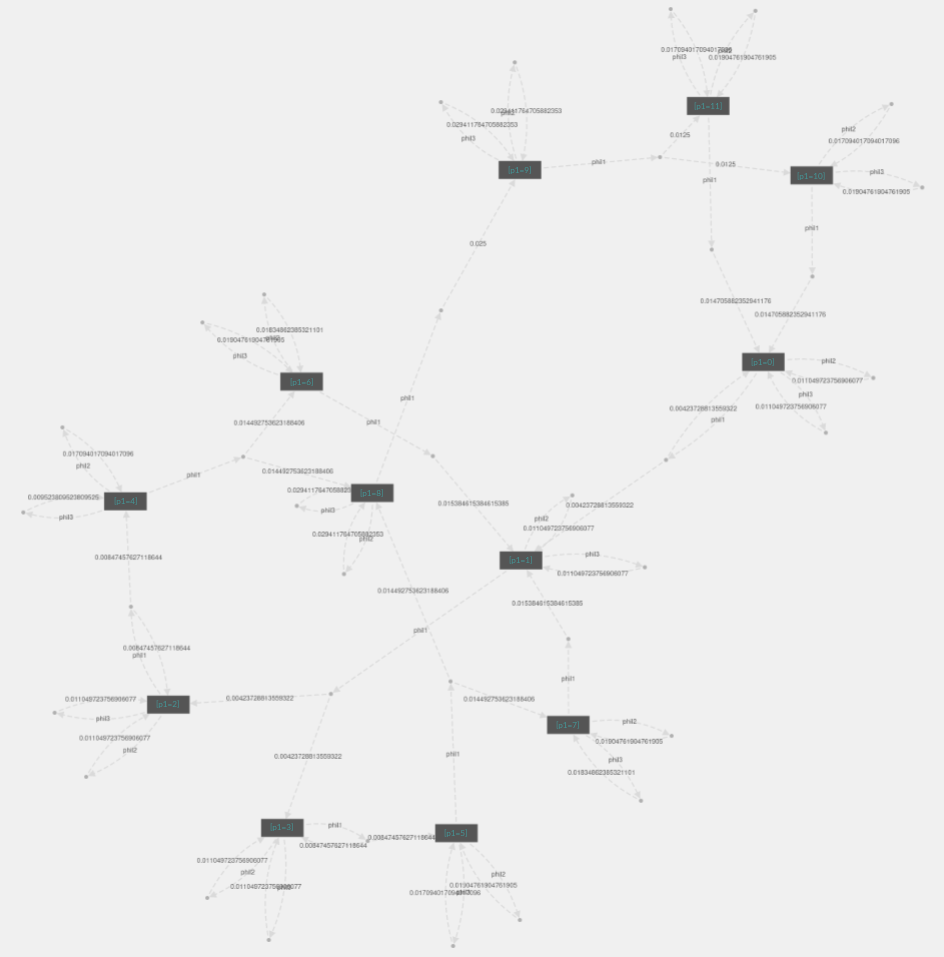
\includegraphics[width=\textwidth]{./06/images/06_01_var.png}
	\caption{\viewNC $\viewparamvalident(\phil{1})$}
	\label{fig:0601var}
\end{figure}

It is also possible to use the view \viewparamvalident to see the interleaved behavior of two or more modules. To see the interleaved behavior of \phil{1} and \phil{2}, we use parallel composition $\viewparamvalident(\phil{1}) \pll \viewparamvalident(\phil{2})$. This results in states $\state_1, \state_2$ being grouped where $(\gfctparamvalident (\state_1 \cond \phil{1}), \gfctparamvalident(\state_1 \cond \phil{2})) = (\gfctparamvalident(\state_2 \cond \phil{1}), \gfctparamvalident(\state_2 \cond \phil{2}))$. Hence only the value of \phil{3} is hidden which results exactly in the desired \redcomment{interleaved model} (Figure \ref{fig:0601var+var}).

\begin{figure}
	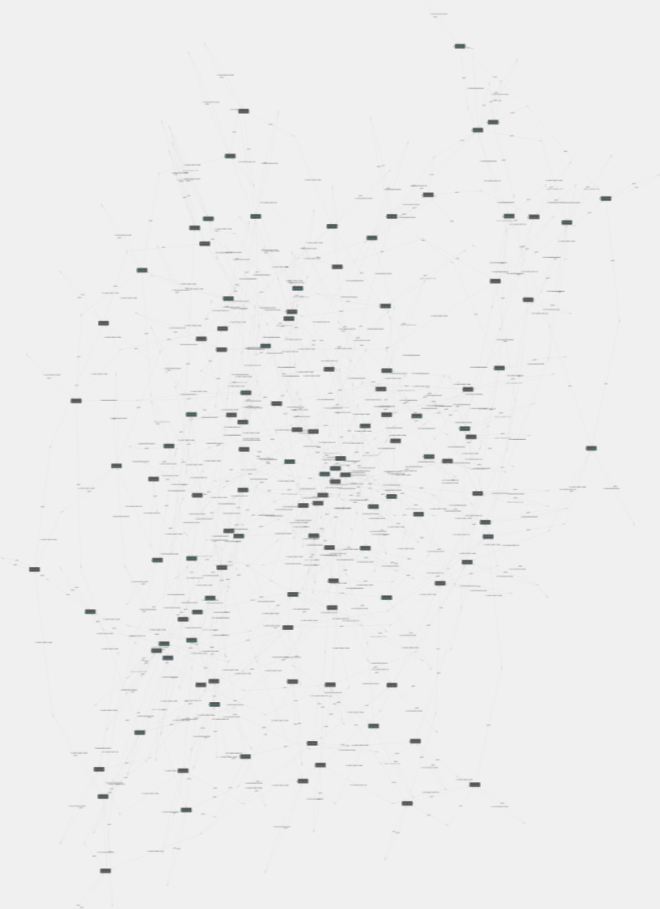
\includegraphics[width=\textwidth]{./06/images/06_01_var+var.png}
	\caption{\viewNC $\viewparamvalident(\phil{1}) \pll \viewparamvalident(\phil{2})$}
	\label{fig:0601var+var}
\end{figure}

In general the views \viewparamdnf and \viewparamcnf are very powerful since they allow arbitrary operations on parameters.

%\begin{itemize}
%	\item USE: dinging Philosopher
%	\item consider dining Philosophers with
%	\item current graphical Representation looks as follows
%	\item only has about 1000 states in case studies prism mdp with about ... states
%	\item in general seems simple
%	\item parameters cluster: allows looking at just one module
%	\item also interleaving of arbitrary modules
%	\item
%	\item hasAction or OutAction-Ident for specific MDP-that run through configuration phases
%	
%\end{itemize}

\subsection{Find out why illegal states is reached}
\newcommand{\critstate}{\mt{\varstyle{2}{2}}}

In this section we want to show how views can be used for debugging. In this specific case we assume that we observed unwanted behavior or model checking results. We know that some states - that is some assignment of variables - are not allowed. We will check if these states are in fact not reachable.

We will consider the following small \mdpN the represents two systems that intend to send information via a unshareable medium. With a probability of $0.8$ a system can establish a connection and with probability of $0.2$ establishing a connection will fail. After an established connection access to the medium shall only be granted, if it is not occupied by the other system. If the medium is not occupied the system starts sending, otherwise it waits until the medium is free. The termination of the transmission is modeled with probabilities. There is 50 percent chance of terminating the transmission and a 50 percent chances of continuing.

The state \critstate should not be reachable, since it represents the situation of the two systems occupying the unshareable medium at the same time. We will check if this state in fact is not reachable by using the $\view[\pptyparamcnf](c(\state))$ where $c(\state) := (x=2) \land (y=2)$ (Figure \ref{fig:0602Var}). Note that we are not using any disregarding \viewN.

\begin{figure}
	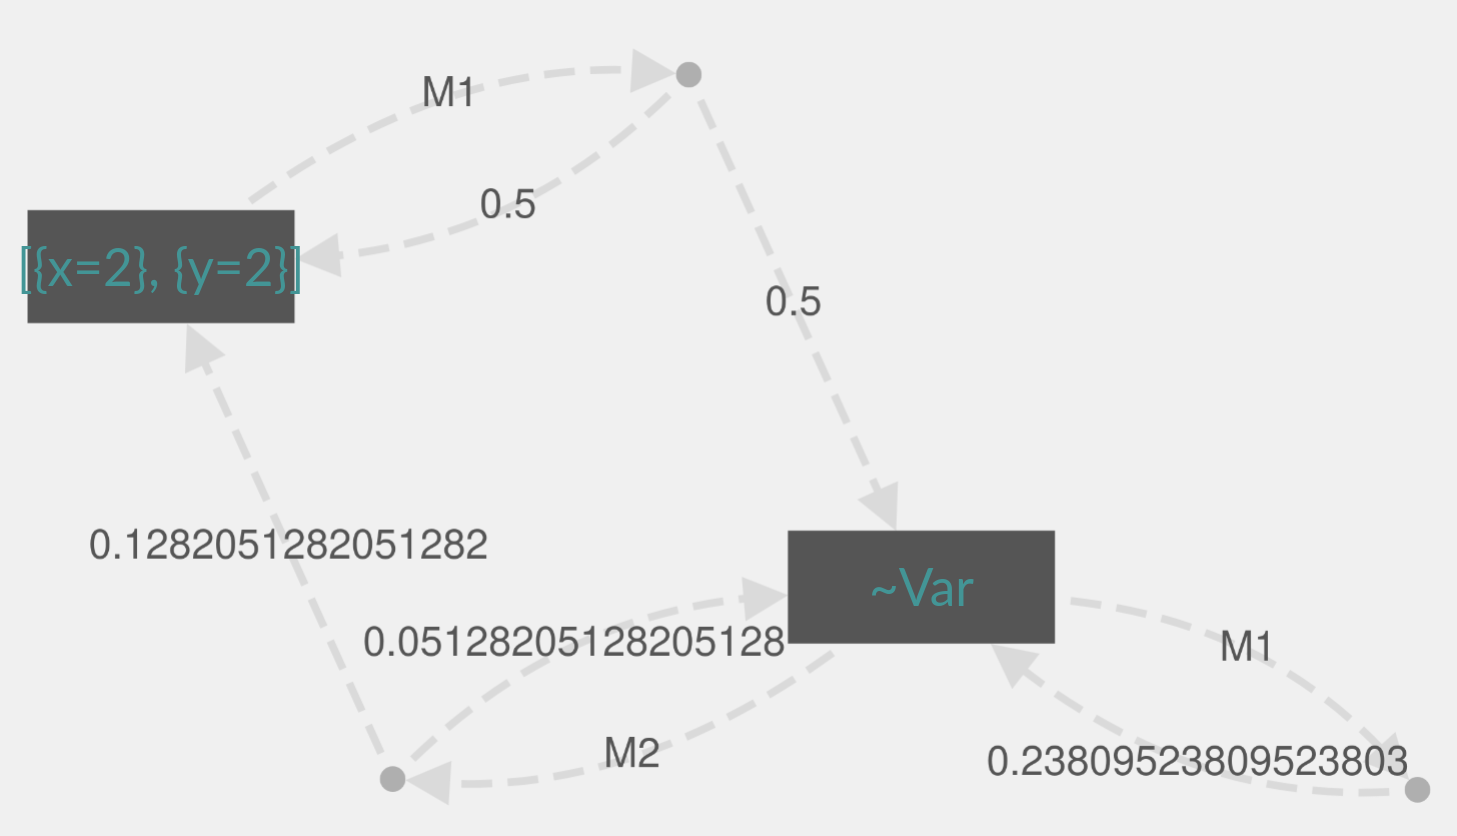
\includegraphics[width=\textwidth]{./06/images/06_02_Var.png}
	\caption{\viewNC $\view[\pptyparamcnf](c(\state))$}
	\label{fig:0602Var}
\end{figure}

We observe, that this state is reachable, because it is shown and only reachable states are shown at all in \pmcvis. The questions occurs how and why. In order to obtain this information it should be investigated by which state this critical state \critstate has been reached. One way of accomplishing that is to look into the database that stores states and transitions. They look as follows. 

An even better approach is to look in the model file, which looks as follows:

Persons with experience in working with prism models, might quickly spot the issue, especially because this is a rather small \mdpN. With less experienced people and especially with larger and more complicated models, finding an issue becomes much more difficult. Hence, let us see how views can help us.

Firstly we will use the view \viewdistance from that state on (Figure \ref{fig:0602VarDistIdDouble} (left)). Because in the current version of the project expansion of grouped states to the ones they contain on a visual level, has not been implemented yet, we will use a custom \viewN that emulates this feature.

%\begin{figure}
%	\begin{minipage}{.5\textwidth}
%%	\begin{subfigure}
%	\centering 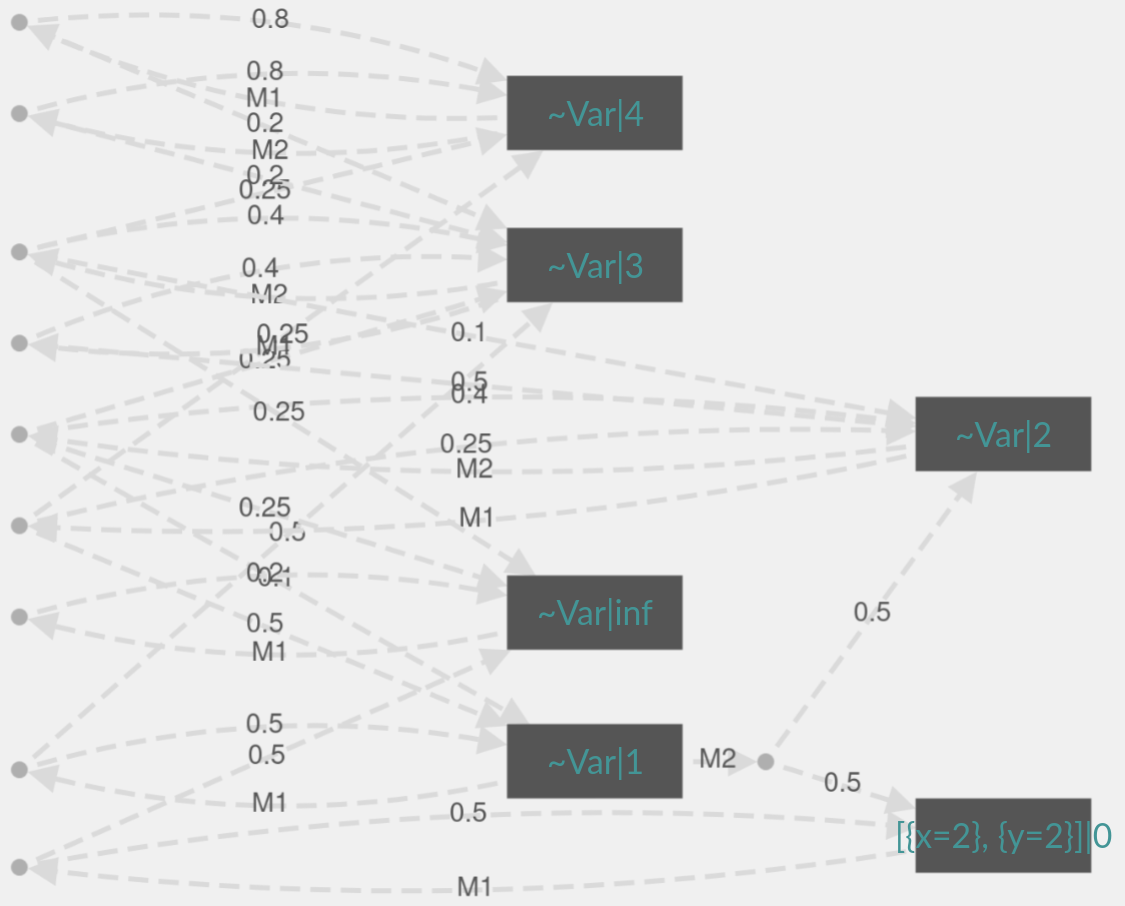
\includegraphics[width=.95\linewidth]{./06/images/06_02_Var+Dist.png}
%	\label{fig:0602Var+Dist}
%%	\caption{\viewNC $\view[\pptyparamcnf](c(\state)) \pll \viewdistance$}
%%\end{subfigure}
%\end{minipage}
%\begin{minipage}{.5\textwidth}
%%	\begin{subfigure}
%	\hspace{10mm}
%	\centering 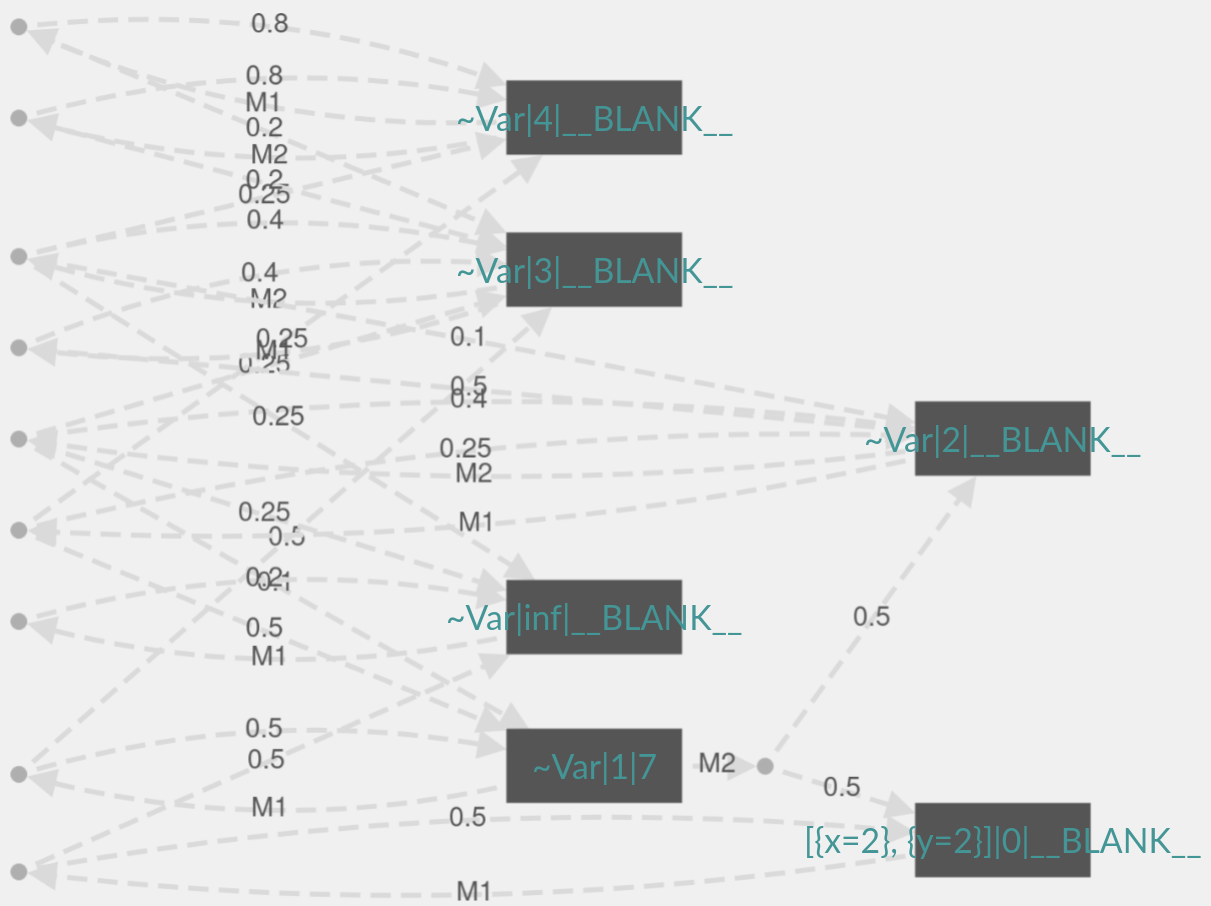
\includegraphics[width=\linewidth]{./06/images/06_02_Var+Dist+Id.png}
%	\label{fig:0602Var+Dist+Id}
%%	\caption{\viewNC $\viewNC \view[\pptyparamcnf](c(\state)) \pll \viewdistance \pll \viewident$}
%%\end{subfigure}

	
%\end{minipage}
%\label{fig:0602VarDistIdDouble}
%%\caption{\viewNC $\view[\pptyparamcnf](c(\state)) \pll \viewdistance$ on the left and \viewN $\view[\pptyparamcnf](c(\state)) \pll \viewdistance \pll \viewident$}
%\end{figure}

\begin{figure}
	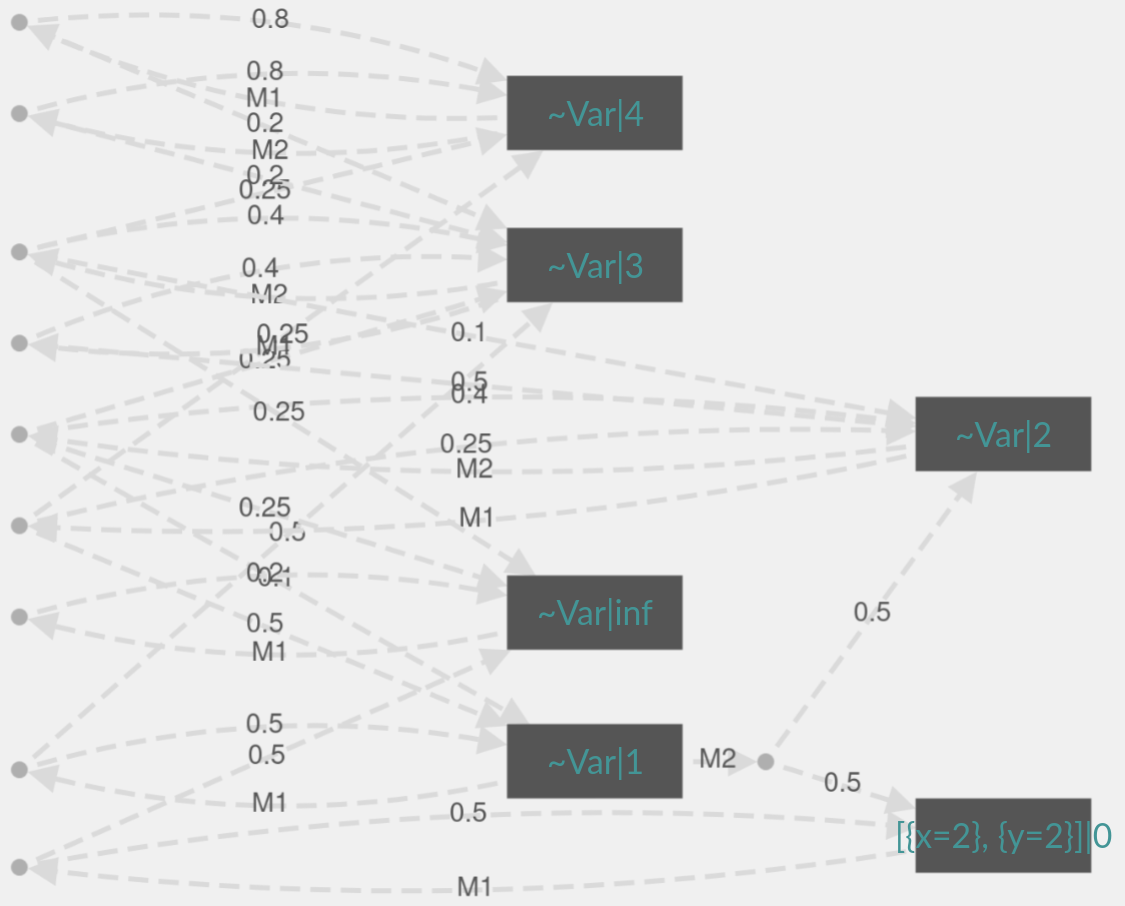
\includegraphics[width=\textwidth]{./06/images/06_02_Var+Dist.png}
	\caption{\viewNC $\view[\pptyparamcnf](c(\state)) \pll \viewdistance$}
	\label{fig:0602Var+Dist}
\end{figure}

\begin{definition}
	Let $\chgph = \chgphtuple$ be \achgphN, $\smstates \subseteq \states$ and $n \in \natnums$. The \viewN \viewident is defined by its \grpfctN \gfctident where $\gfctsubident : \smstates \to \imggrp$ with
	\[
	\gfctsubident(\state) = \state
	\]
	and $\imggrp = \states \cup \remset$.
\end{definition}

\sloppy
We will use partial application with $ \view[\pptyparamcnf](c(\state)) \compselect \viewident$ where $\compselectset = \{(\gfctdistance,1)\}$ to expand that state. The MDP-Graph then looks as in \ref{fig:0602Var+Dist+Id}. It is to see that the state only contains a single state namely with the id seven. In the current version of implementation it is not possible, to obtain the parameter values. With the database file we obtain that this is the state where $x=2$ and $y=1$. Because $x=2$ represents the system 1 one sending and system 2 waiting, we see that is possible for the second  system to begin to send on the medium although it is already occupied by the first system!

\begin{figure}
	\centering 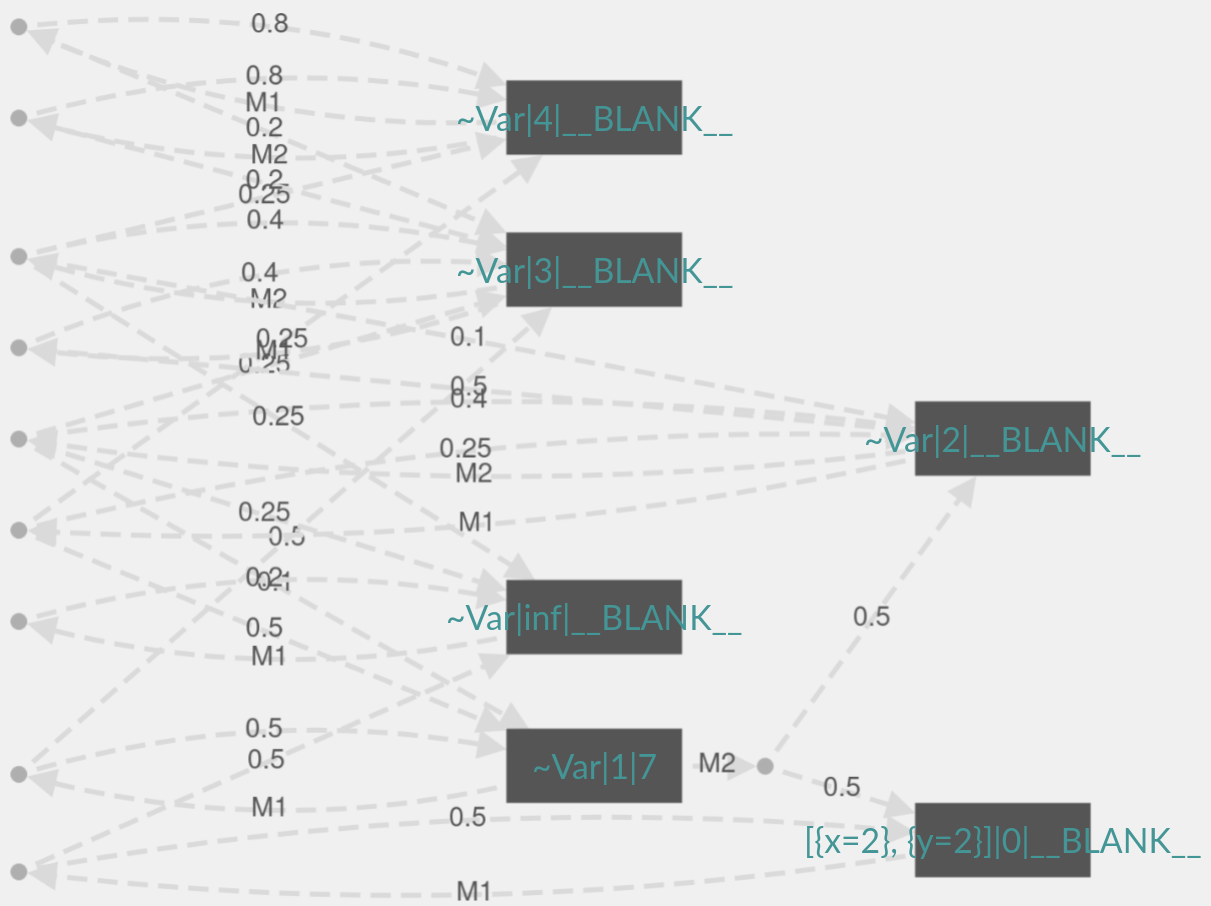
\includegraphics[width=\textwidth]{./06/images/06_02_Var+Dist+Id.png}
	\caption{\viewNC $\viewNC \view[\pptyparamcnf](c(\state)) \pll \viewdistance \compselect \viewident$ where $\compselectset = \{(\gfctdistance,1)\}$}
	\label{fig:0602Var+Dist+Id}
\end{figure}

When now looking at the prism file we can see why this is the case. In line when $y=1$ there is a 50 percent chance to enter $y=2$. This line originally was intended for termination of the transmission. From $y=1$ it should not be possible to enter $y=2$ if $x=2$. After fixing this, the state no longer appears after the application of $\viewparamdnf(c(\state))$

	
%\begin{itemize}
%	\item USE: two process switch 
%	\item illegal state has been reached?
%	\item given state 2,2 should not be reachable
%	\item is reachable
%	\item is only!
%	\item apply distance cluster
%	\item emulate not yet feature of expansion
%	\item use identityView (with Parameters)
%	\item see in Database
%	\item fix in File
%\end{itemize}


%\subsection{Find out how why we reach a certain state}
%%	\item two dies
%%	\item property cluster

\subsection{Understand and Debug \chgphN}

In this subsection we want to take a look at a more complex usecase how views might help us to understand and fix a given \mdpN. We refer to the \mdp \redcomment{reference}.

Firstly, we will gather some understanding of the model. We already saw in chapter ch that variables can help a lot with understanding an \chgphN. When applying $\viewparamvalident(\texttt{time})$ we see that the \chgphN has a limited timed behavior (Figure \ref{fig:0603time_phases} left). When applying $\viewparamvalident(\texttt{phases})$ we observe that the system is operating in phases (Figure \ref{fig:0603timeandphases} right). If we consider $\viewparamvalident(\texttt{time}) \pll \viewparamvalident(\texttt{phases})$ we see that the phases are repeated for each iteration of time (Figure \ref{fig:0603time+phases} right). However, we still don not have any information about the behavior of the system in these phases. Since this model has actions we will consider the \viewN \viewweakoutactident (Figure \ref{fig:0603act}). We obtain that we have sets of states which only have transitions with the action \texttt{[reconfigure]} outgoing, the action \texttt{[working]} outgoing, the actions \texttt{[configure1]} outgoing, \texttt{[configure2]}, \texttt{[end\_reconfigure]}, the action \texttt{[working]} outgoing or the action \texttt{[end]} outgoing \redcomment{Figure}. By interpreting the name of the actions we see that this system seems to have a configuration phase a working phase a reconfiguring phase and an end phase. The grouping appears to be very similar to \viewparamvalident(\texttt{phases}). Hence, we consider $\viewweakoutactident \pll \viewparamvalident(\texttt{phases})$ (Figure \ref{fig:0603act+phases}). Indeed the enumeration coincides with the grouping of outgoing actions, with the exception of \texttt{[end]} and \texttt{[reconfigure]} \redcomment{timed behavior?}

\begin{figure}
	\begin{subfigure}{.5\textwidth}
		\centering 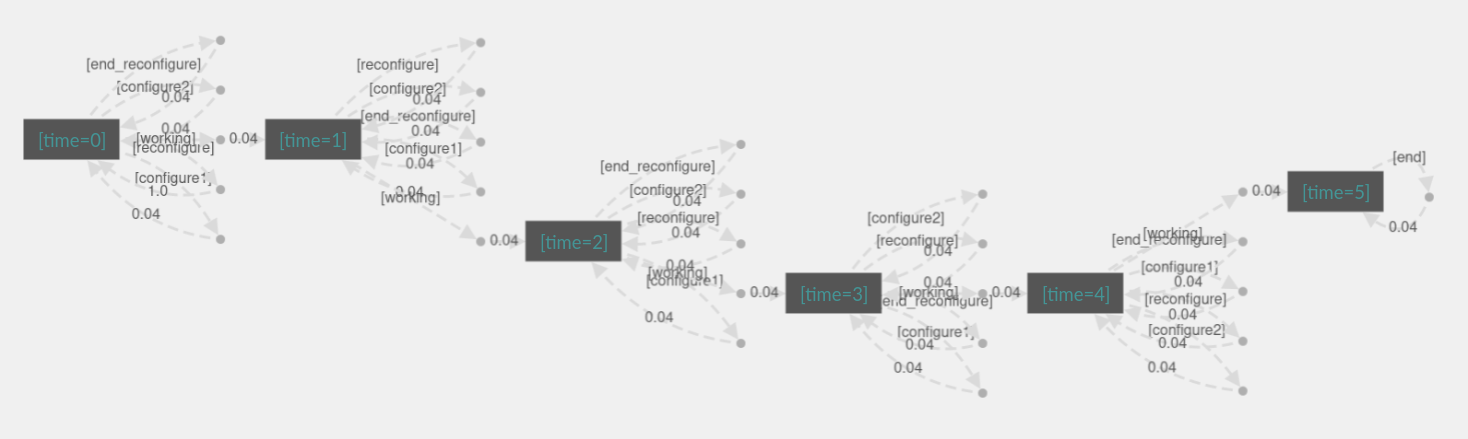
\includegraphics[width=\textwidth]{./06/images/06_03_time.png}
%		\label{fig:0601time}
%		\caption{\viewNC $\viewNC \view[\pptyparamcnf](c(\state)) \pll \viewdistance \compselect \viewident$ where $\compselectset = \{(\gfctdistance,1)\}$}
	\end{subfigure}
	\hspace{5mm}
	\begin{subfigure}{.5\textwidth}
		\centering 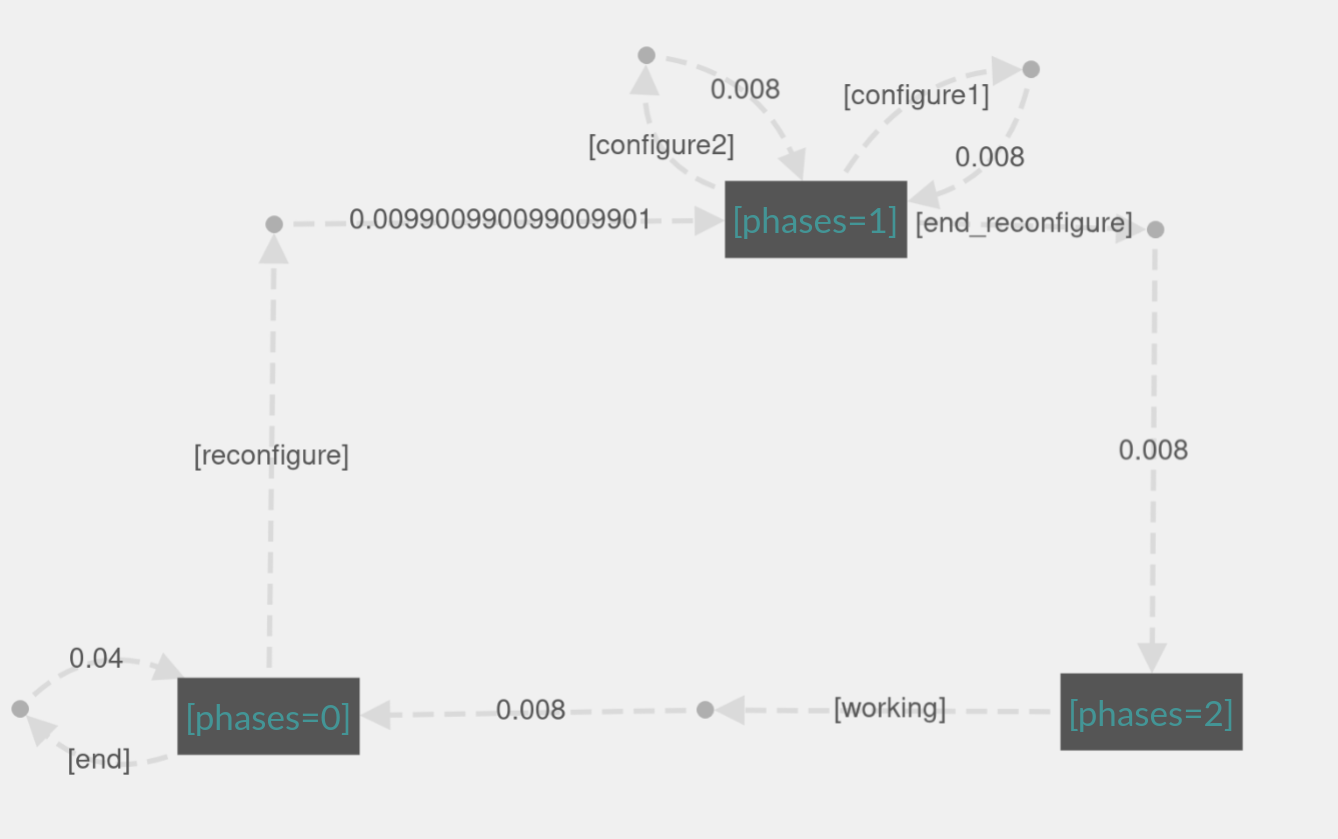
\includegraphics[width=\textwidth]{./06/images/06_03_phases.png}
%		\label{fig:0601phases}
%		\caption{\viewNC $\viewNC \view[\pptyparamcnf](c(\state)) \pll \viewdistance \compselect \viewident$ where $\compselectset = \{(\gfctdistance,1)\}$}
	\end{subfigure}
	\caption{\viewNC $\viewparamvalident(\texttt{time})$ (left) and \viewN $\viewparamvalident(\texttt{phases})$ (right)}
	\label{fig:timeandphases}
\end{figure}

\begin{figure}
	\centering 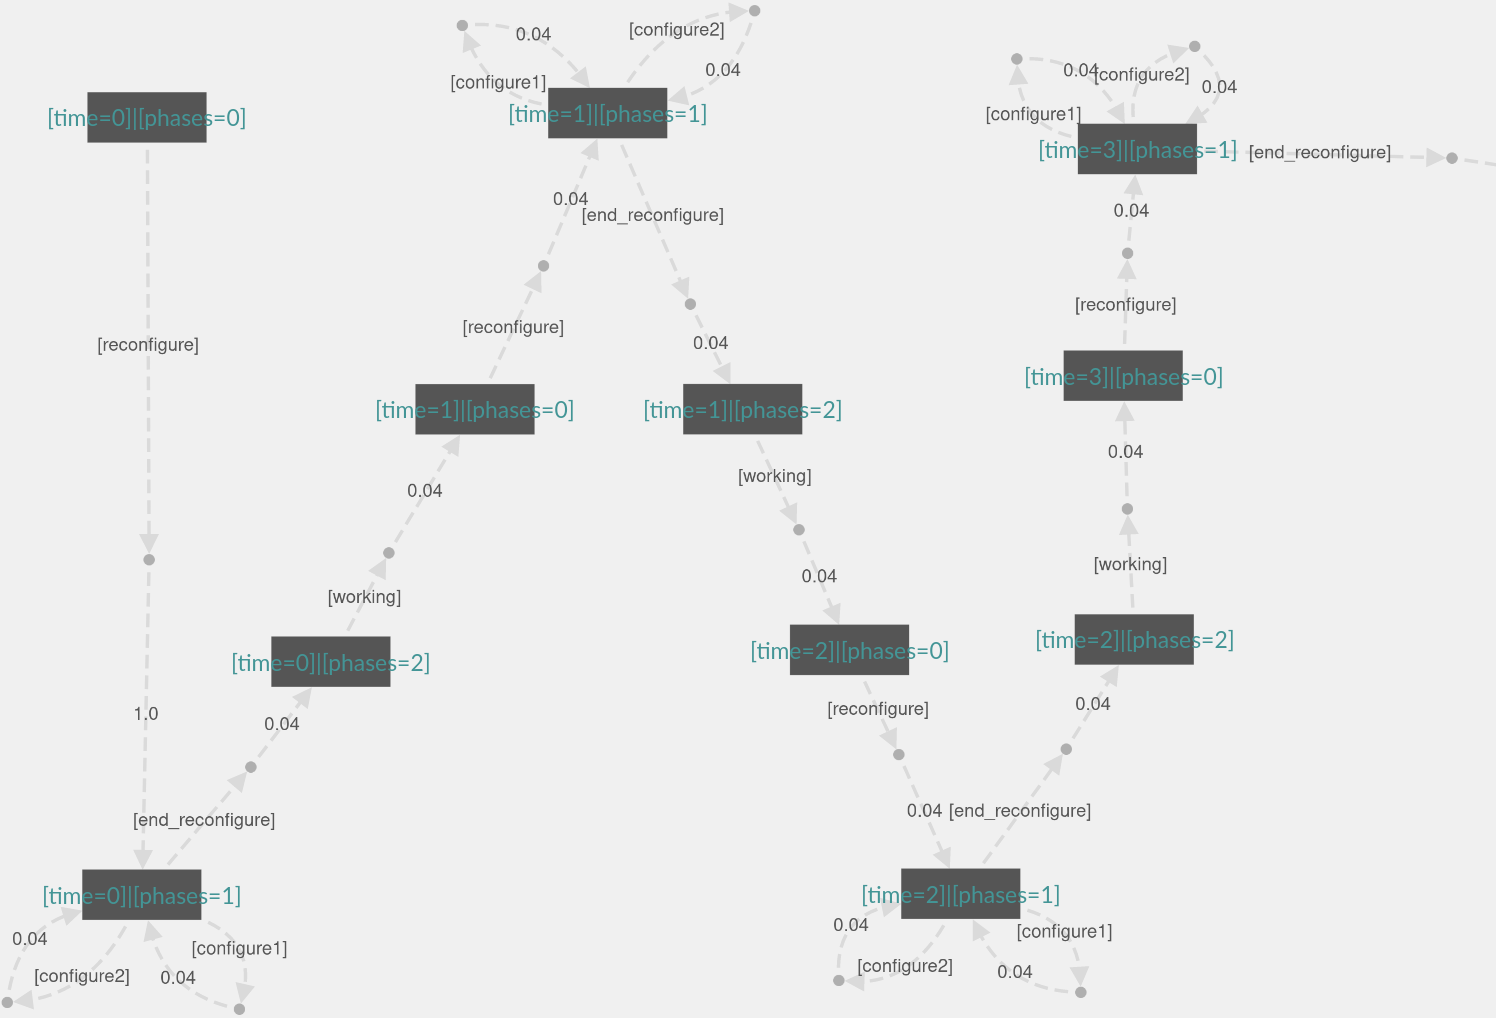
\includegraphics[width=\textwidth]{./06/images/06_03_time+phases.png}
	\caption{\viewNC $\viewparamvalident(\texttt{time}) \pll \viewparamvalident(\texttt{phases})$}
	\label{fig:0603time+phases}
\end{figure}

\begin{figure}
	\centering 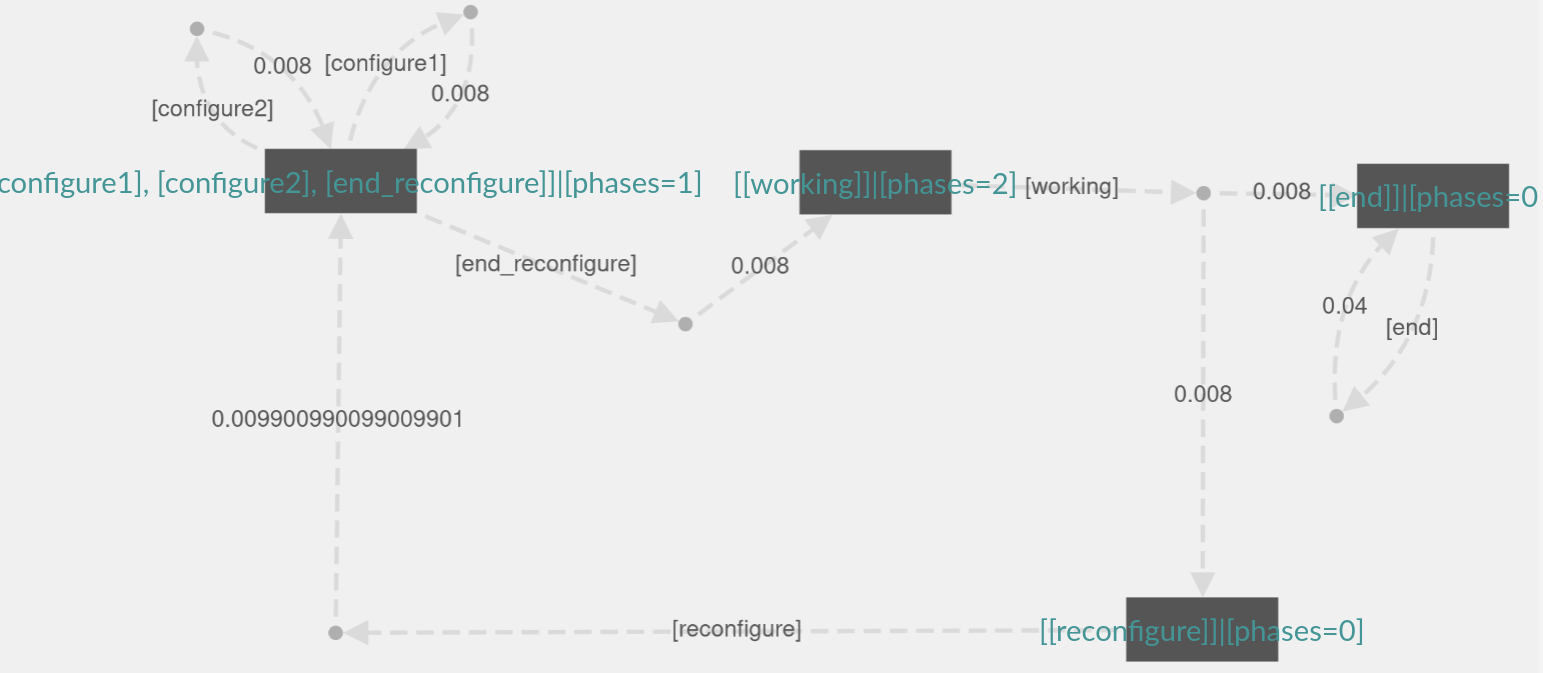
\includegraphics[width=\textwidth]{./06/images/06_03_act.png}
	\caption{\viewNC \viewweakoutactident}
	\label{fig:0603act}
\end{figure}

\begin{figure}
	\centering 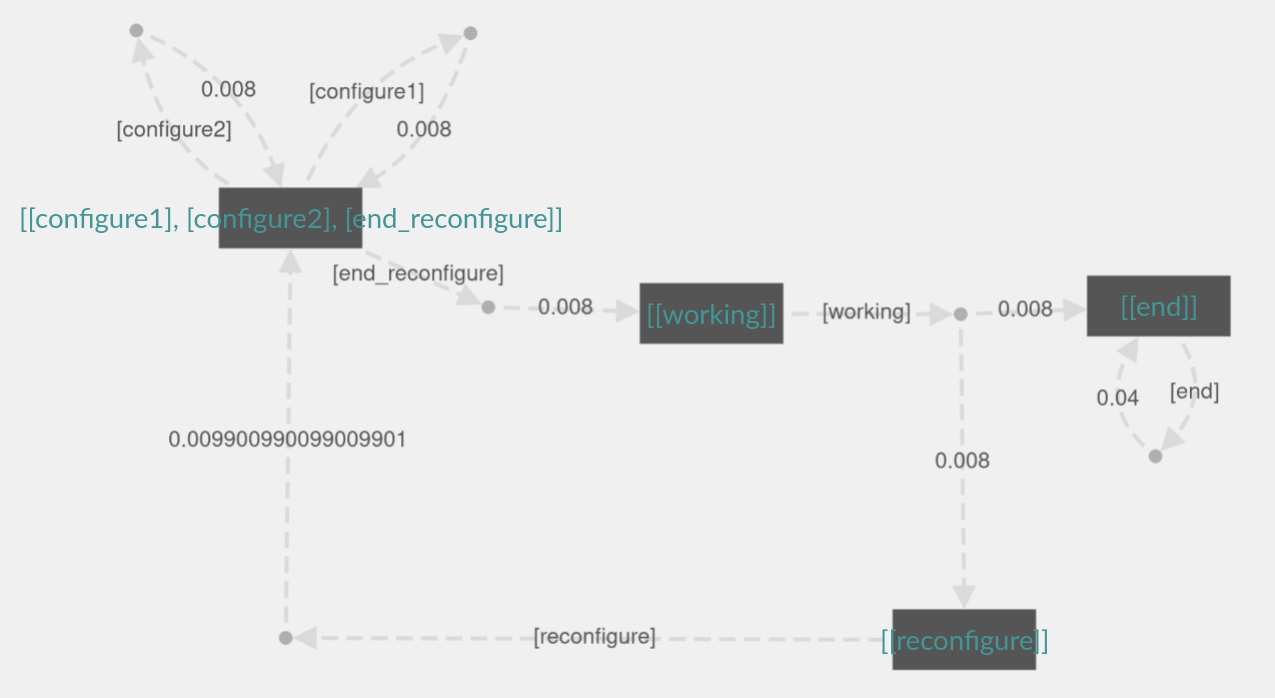
\includegraphics[width=\textwidth]{./06/images/06_03_act+phases.png}
	\caption{\viewNC $\viewparamvalident(\texttt{time}) \pll \viewparamvalident(\texttt{phases})$}
	\label{fig:0603act+phases}
\end{figure}

Hence we know that the system is working for $\texttt{phase}=0$, configuring for $\texttt{phase}=1$ and termination configuration in $\texttt{phase}=2$. This process is repeated six times until $\texttt{time}=5$.

In general we learned that this system runs several times with choosing certain configurations each time before it runs. Its reward function rewards states that work with a better configuration. A classic model checking \redcomment{value} is to determine \redcomment{MIN EXP REWARD} and \redcomment{MAX EXP REWARD}. For \redcomment{MIN EXP REWARD} we obtain \redcomment{x}, for \redcomment{MAX EXP REWARD} \redcomment{inf}. Since the system is modeled for a finite time and each time chooses from a finite set of configurations, it is unwanted behavior, that \redcomment{MAX EXP REWARD} is infinite. We will now show how views can help to find the cause.

Such behavior of infinite \redcomment{MAX EXP REWARD} is often caused by cycles. A feasible idea would be to use a view with cycles. As it will be discussed in Chapter \redcomment{Performance} these \viewsN very ressource intensive when there are larger strongly connected components. Moreover when finding strongly connected components the cycles are equally found since each cycle is a strongly connected component. The view \viewscc yields that there are quite large strongly connected components (Figure \ref{fig:0603scc}). To find out where these are locate we consider the parallely composed \viewN on \mdpN with $\viewscc \pll \viewweakoutactident$ (Figure \ref{fig:0603scc+act}). We see that the strongly connected components are in the configuring phase. When taking a look at the prism file, we see that we can arbitrarily often switch the configuration. Hence, it is not assured that a configuration can only be selected once. This causes infinite paths in the \mdpN, which in consequence cause infinite maximal expectations. This can be fixed by assuring that a configuration can only be selected once. An easy way of accomplishing this is to sequentialize the selection of the two configurations: Firstly \texttt{[configuration1]} is selected, afterwards \texttt{[configuration2]} and finally the configuration phase ends (\texttt{[end\_configuration]} is the only available action left to take).

\begin{figure}
	\centering 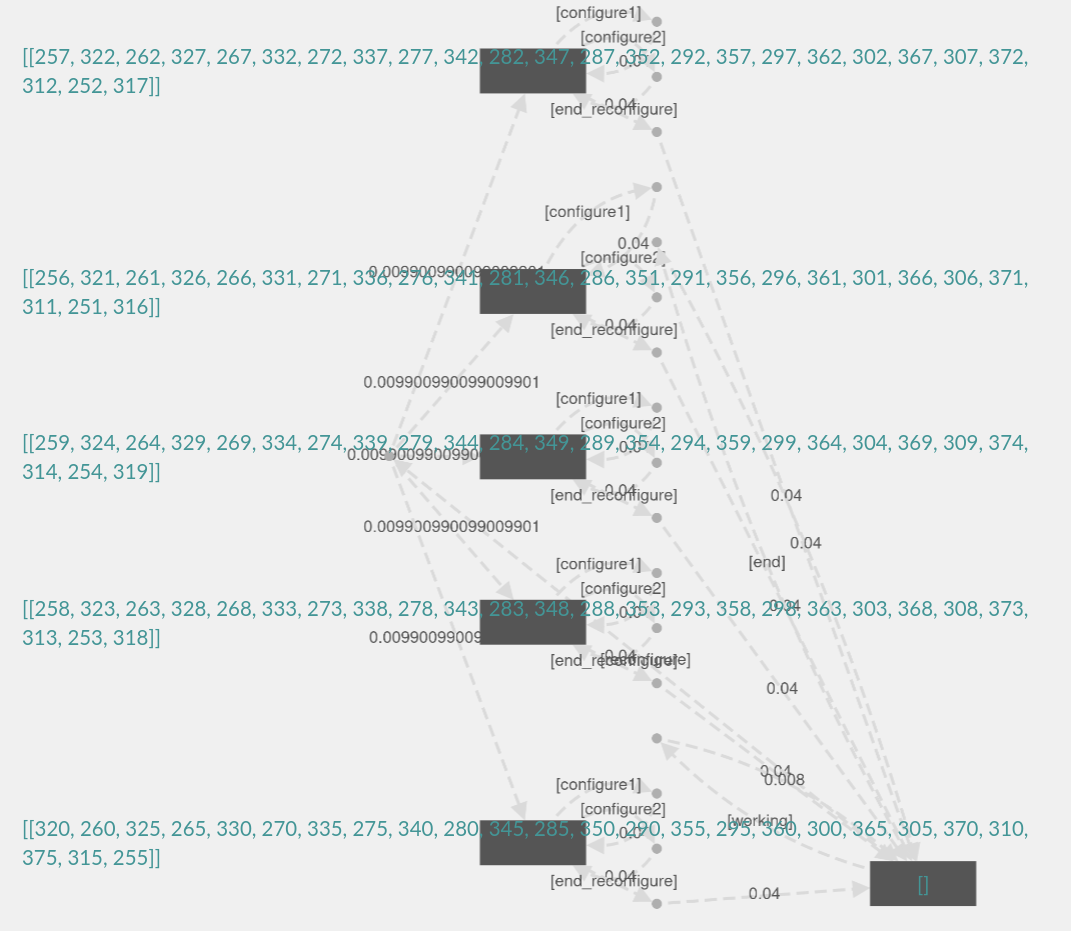
\includegraphics[width=\textwidth]{./06/images/06_03_scc.png}
	\caption{\viewNC \viewscc}
	\label{fig:0603scc}
\end{figure}

\begin{figure}
	\centering 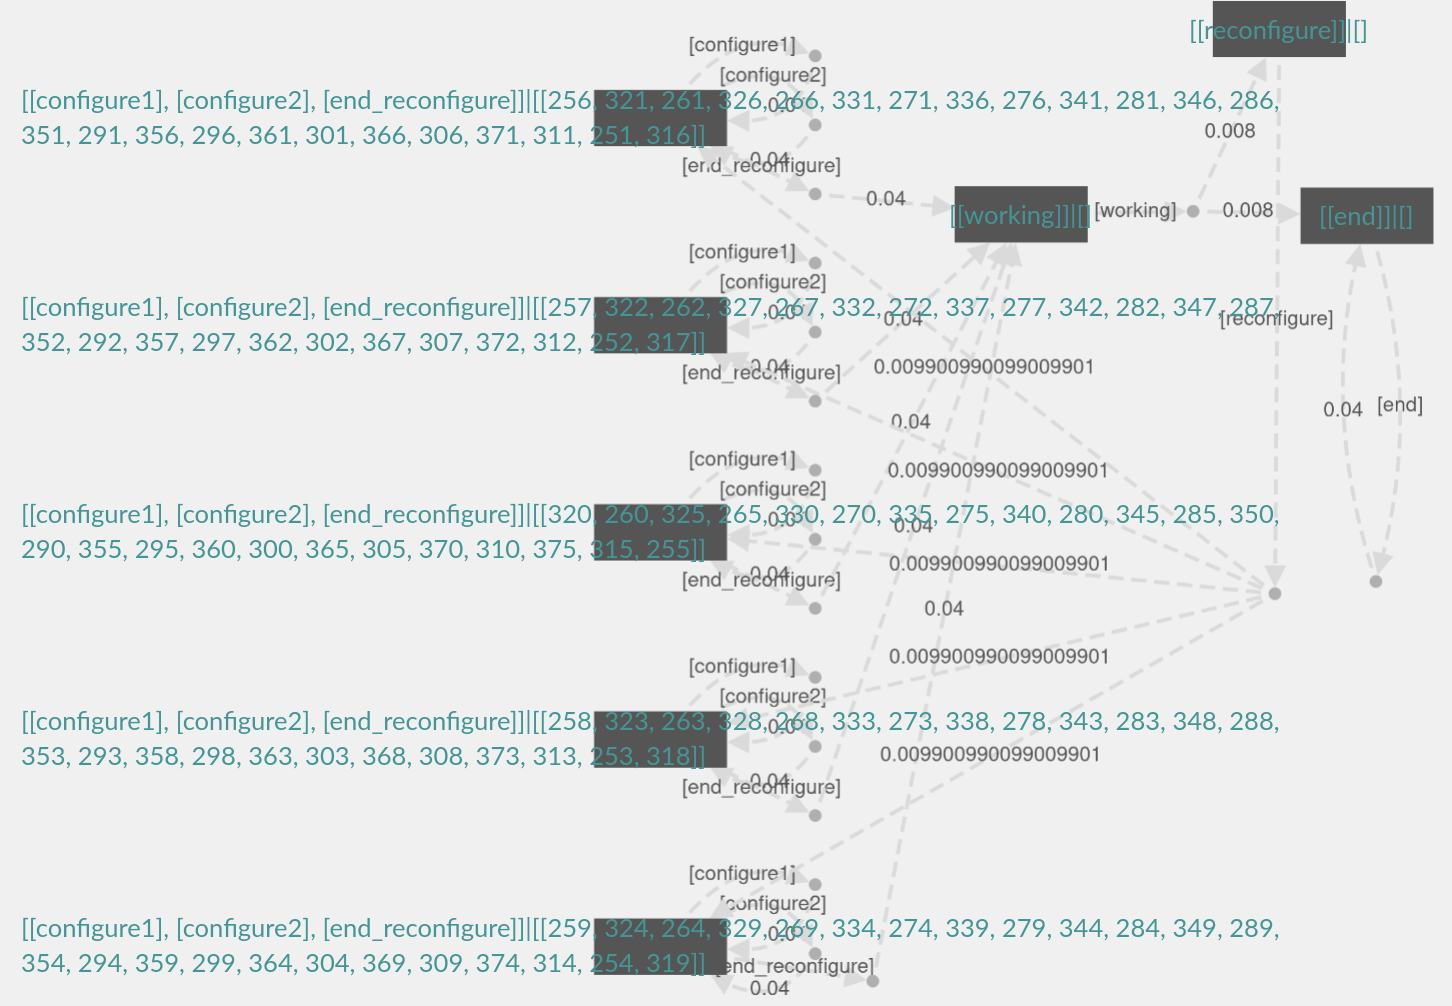
\includegraphics[width=\textwidth]{./06/images/06_03_scc+act.png}
	\caption{\viewNC $\viewscc \pll \viewweakoutactident$}
	\label{fig:0603scc+act}
\end{figure}

%\begin{itemize}
%	\item USE: scc with loops
%	\item We already saw in chapter ch that variables can help a lot with understanding an \chgph
%	\item When applying it to time and phases we see that the system has limited timed behavior and that it operates in phases
%	\item considering time pll phases we see that these phases are repeated for each time
%	\item Still no idea what the model actually does
%	\item since this view has actions it may help to use the outactions view
%	\item see phases
%	\item when activating phases pll action see that in phase=0 ... and will eventually terminate in phase=0
%	\item \redcomment{time+scc+init}
%%	\item time apply strongly connected components -> structure of mdp very clear
%%	\item apply init to see where it start
%	\item maxReward is infinite -> not wanted
%	\item search for cycles or scc
%	\item are cycles $\to$ exact cycles \redcomment{maybe exact cycles}
%	\item fix mdp $\to$ no more cycles $\to$ show no more cycles
%	
%\end{itemize}

\subsection{Performance}

\viewsNC shall be used on \mdpsN that may have millions of states. For this reason in this section we will consider the time to create a new view. In addition we will take a look at the build time of internal graph structure (\texttt{mdpGraph}) that is based on the \jgrapht library, with respect to its built time and memory occupation. The tests have been performed on a Dell XPS 9370 (16 GB RAM, i7-8550U) with Manjaro KDE. Only neccesary tools where opened when the test were running: Firefox and IntelliJ.

Time was measured with self written class \texttt{Timer} which utilizes the package \texttt{java.time.LocalTime}. Class implementation and sample usecase are provided in the appendix \redcomment{to be added in the appendix}. Memory occupation has been measured with with the tool Java Object Layout (JOL) provided by openJDK. The method used was \texttt{totalSize()} in \texttt{org.openjdk.jol.info.GraphLayout}. For the benchmark one single scalable \mdpN is used (prism model file in appendix). Sizes considered are 50, 100, 500,1 000, 5 000, 10 000, 50 000, 100 000, 500 000 and 1 000 000. Using one single scalable \mdpN means that execution times and memory occupied might vary with differing graph structure of the \mdpN. This is especially the case for \viewsN based on the graph structure. Hence  in this section we will give more of an overview of the expected values for creation times and memory occupation rather than a detailed analysis.

Firstly we will consider the time required to create \viewsN. All \viewsN are created 100 times for each considered size of the \mdpN. Their execution times for each sizes then are averaged. As we know from Chapter \ref{ch:viewimpl} creating a view involves to instantiate the object and execute the build function. The instantiation only involves setting a hand full of private attributes. Since the amount of attributes of a view is fix and their size does not cohere with the size of the \mdpN, the is instantiation time is negligible. Building \texttt{mdpGraph} is also part of instantiating a \viewN in case it has not yet been built on the model, but will be considered separately. Hence, we will focus on the time occupied by the \texttt{buildView()} method. As we know from section \ref{ch:viewimpl} the build \texttt{buildView()} method splits into four parts: 1) checking prerequisites ("prechecks"), 2) creating a new column, 3) executing \grpfctN 4) write results to database. Firstly we will consider the computation time for the grouping function as the time actions performed in the steps 1) 2) and 4) are almost identical or identical.
	
In Figure \ref{fig:grpfcttimes} we see the averaged execution times (100 executions) of \texttt{groupingFunction} for the different \viewsN. It is to see that the execution times overall are very similar and behave linear to the amount of states of the \mdpN. For \mdpsN with up to 1 million states for no \viewN the execution time of its grouping function exceeds 1.5 seconds. Variation in the magnitude of microseconds with very small \mdpsN are to be expected. In general the performance results as shown indicates very good scalability with respect of views being usable on large models. This very good performance is to large portion attributed to the graphstructure provided by \jgrapht.

In Figure \ref{fig:compdbgraphgrpfct} we see the execution time of the grouping function compared to executing the generated SQL statements (writing results/mappings to database) and the creation of the \texttt{mdpGraph}. We see that apart from prechecks, the execution time of the grouping function is the least time consuming operation. Most time is taken by writing the results to the database, where even building the \texttt{mdpGraph} is faster. Times for writing to the database, refer to the at this time present implementation of the database of \pmcvis which might be subject to changes in the future.

As stated before the performance of computing grouping functions that quickly heavily rely on the implemented graph structure (\texttt{mdpGraph}). This graph structure is held in memory and become quite large for \mdpsN with about one million states. The \redcomment{Figure} displays the measured deep size (including referenced objects) of the \texttt{mdpGraph}. As one would expect the size of the \texttt{mdpGraph} is linear to the size of the \mdpN. Additionally, it can be seen that up to 1.3 GB of memory are occupied for the graph alone if, the \mdpN reaches about 1 million states. Depending on the operating system, the amount of memory built into the machine (PC) and the currently available memory, it is possible to utilize the \texttt{mdpGraph} even for large \mdpsN. Still it is to be kept in mind that this only is the size of the built graph object. When reading from the database in order to build the \texttt{mdpGraph} more memory is needed as objects containing the information from the database also temporarily stay in memory. \pmcvis itself will also require memory as other possibly unrelated process that run on the system. On the machine used for testing, building the \texttt{mdpGraph} for \mdpsN with about 1 million states and creating views on them was still reasonable, while at the same time also close to the memory limitation of the system.

In general we conclude that computation of grouping functions is rather quick and scalable. Building times of the \texttt{mdpGraph} are reasonable, but entails heavy memory utilization. Database accesses are the most time consuming fraction of the time needed to create a view. 

\begin{figure}
	\begin{tikzpicture}
	\begin{loglogaxis}
		[
		width=\textwidth,
		height=8cm,
		xlabel={State amount},
		ylabel={$\frac{time}{ms}$},
		legend pos=north west,
		ymin=0,
%		ymax=1000,  % Adjust the y-axis range as needed
		]
		
		\addplot table [x=StateCount, y=0AvgG, col sep=comma] {./06/PerformanceTests/GroupingFunction/InActIdentView.csv};
		\addplot table [x=StateCount, y=0AvgG, col sep=comma] {./06/PerformanceTests/GroupingFunction/OutActIdentView.csv};
		\addplot table [x=StateCount, y=0AvgG, col sep=comma] {./06/PerformanceTests/GroupingFunction/InActView.csv};
		\addplot table [x=StateCount, y=0AvgG, col sep=comma] {./06/PerformanceTests/GroupingFunction/OutActView.csv};
		\addplot table [x=StateCount, y=0AvgG, col sep=comma] {./06/PerformanceTests/GroupingFunction/OutActSetSizeView.csv};
		\addplot table [x=StateCount, y=0AvgG, col sep=comma] {./06/PerformanceTests/GroupingFunction/VariablesView.csv};
		\addplot table [x=StateCount, y=0AvgG, col sep=comma] {./06/PerformanceTests/GroupingFunction/VariablesViewDnf.csv};
		\addplot table [x=StateCount, y=0AvgG, col sep=comma] {./06/PerformanceTests/GroupingFunction/VariablesViewCnf.csv};
		\addplot table [x=StateCount, y=0AvgG, col sep=comma] {./06/PerformanceTests/GroupingFunction/ReachabilityView.csv};
		\addplot table [x=StateCount, y=0AvgG, col sep=comma] {./06/PerformanceTests/GroupingFunction/DistanceView.csv};
		\addplot table [x=StateCount, y=0AvgG, col sep=comma] {./06/PerformanceTests/GroupingFunction/SccView.csv};
		\addplot table [x=StateCount, y=0AvgG, col sep=comma] {./06/PerformanceTests/GroupingFunction/SccbView.csv};
		\addplot table [x=StateCount, y=0AvgG, col sep=comma] {./06/PerformanceTests/GroupingFunction/APView.csv};
		\addplot table [x=StateCount, y=0AvgG, col sep=comma] {./06/PerformanceTests/GroupingFunction/InitView.csv};
		\addplot table [x=StateCount, y=0AvgG, col sep=comma] {./06/PerformanceTests/GroupingFunction/PropertyView.csv};


		
%		\legend{InActIdentView, 
%			OutActIdentView,
%			InActView,
%			OutActView,
%			OutActSetSizeView,
%			VariablesView,
%			VariablesViewDnf,
%			VariablesViewCnf, 
%			ReachabilityView, 
%			DistanceView,
%			SccView,
%			SccbView,
%			APView,
%			InitView,
%			PropertyView}

	\end{loglogaxis}
\end{tikzpicture}
	\caption{Average grouping function computation times}
	\label{fig:grpfcttimes}
\end{figure}


\begin{figure}
	\begin{tikzpicture}
	\begin{loglogaxis}
		[
		width=\textwidth,
		height=8cm,
		xlabel={State amount},
		ylabel={$\frac{time}{ms}$},
		legend pos=north west,
		ymin=0,
		%		ymax=1000,  % Adjust the y-axis range as needed
		]
		
	
		\addplot table [x=StateCount, y=0AvgG, col sep=comma] {./06/PerformanceTests/GroupingFunction/OutActIdentView.csv};
		\addplot table [x=StateCount, y=0AvgMdp, col sep=comma] {./06/PerformanceTests/MdpGraph/MdpGraph.csv};
		\addplot table [x=StateCount, y=0AvgE, col sep=comma] {./06/PerformanceTests/ExecuteBatch/ExecuteBatchInActIdentCSV2-all.csv};
		
		
		
		
		\legend{Grouping Function, 
				Create MDP Graph,
				Write to Database
			}
		
	\end{loglogaxis}
	\end{tikzpicture}
	\caption{Average times for grouping function computation (1 representative from Figure \ref{fig:grpfcttimes}), writing to the database and building the \texttt{mdpGraph}}
	\label{fig:compdbgraphgrpfct}
\end{figure}


\begin{figure}
	\begin{tikzpicture}
		\begin{loglogaxis}
			[
			width=\textwidth,
			height=8cm,
			xlabel={State amount},
			ylabel={$\frac{time}{ms}$},
			legend pos=north west,
			ymin=0,
			%		ymax=1000,  % Adjust the y-axis range as needed
			]
			
			
			\addplot table [x=StateCount, y=MdpSizeByte, col sep=comma] {./06/PerformanceTests/MdpGraph/MdpGraphSize.csv};
			
				
%			\legend{BuildTimeView, 
%				CreateMdpGraph,
%				ExecuteBatch
%			}
			
		\end{loglogaxis}
	\end{tikzpicture}
	\caption{Size of \texttt{mdpGraph} for different model sizes}
	\label{fig:sizemdpgraph}
\end{figure}

\end{document}